\RequirePackage{fix-cm}
\documentclass[smallextended]{svjour3}
\smartqed

\usepackage{amssymb,mathtools,bm}
\usepackage{graphicx}
\usepackage{float}
\usepackage{booktabs}
\usepackage{microtype}
\usepackage{xurl}
\usepackage[square,numbers,sort&compress]{natbib}
\usepackage[hidelinks]{hyperref}
% svjour3 leaves a recursive stub for an undefined chapter counter; clear it
% before cleveref inspects counter-reset lists.
\makeatletter
\let\cl@chapter\relax
\makeatother
\usepackage[nameinlink,capitalise,noabbrev]{cleveref}

\spnewtheorem{assumption}[theorem]{Assumption}{\bfseries}{\rmfamily}
\crefname{assumption}{assumption}{assumptions}
\Crefname{assumption}{Assumption}{Assumptions}
\newcommand{\R}{\mathbb{R}}
\newcommand{\N}{\mathbb{N}}
\newcommand{\cF}{\mathcal{F}}
\newcommand{\cT}{\mathcal{T}}
\newcommand{\cC}{\mathcal{C}}
\newcommand{\cP}{\mathcal{P}}
\newcommand{\ip}[2]{\langle #1,#2\rangle}
\newcommand{\norm}[1]{\lVert #1\rVert}
\newcommand{\eps}{\varepsilon}
\DeclareMathOperator{\rank}{rank}
\DeclareMathOperator{\diag}{diag}
% Generated from the frozen transcript-PEP and accounting payloads.
\newcommand{\TranscriptCases}{2,000}
\newcommand{\JointAcceptCount}{896}
\newcommand{\JointAcceptRate}{44.8\%}
\newcommand{\RectangleAcceptCount}{160}
\newcommand{\RectangleAcceptRate}{8.0\%}
\newcommand{\TwoBinAcceptCount}{338}
\newcommand{\TwoBinAcceptRate}{16.9\%}
\newcommand{\FourBinAcceptCount}{487}
\newcommand{\FourBinAcceptRate}{24.3\%}
\newcommand{\TwoBinRecoveredDependencePct}{24.2\%}
\newcommand{\FourBinRecoveredDependencePct}{44.4\%}
\newcommand{\JointOnlyCount}{736}
\newcommand{\JointOnlyRate}{36.8\%}
\newcommand{\JointViolationCount}{0}
\newcommand{\MedianRectangleGap}{4.0}
\newcommand{\MeanRectangleGap}{10.365}
\newcommand{\MedianJointOnlySlack}{0.463}
\newcommand{\PepCells}{36}
\newcommand{\PepPositiveCells}{3}
\newcommand{\PepAmbiguousCells}{4}
\newcommand{\PepOffShiftCells}{0}
\newcommand{\TranscriptPayloadHash}{5b7fe99bfa34c07d0252582244f22d27df3f32f8d2cd93ced08b8df369dd5597}
\newcommand{\ProxyHorizonMin}{15}
\newcommand{\ProxyHorizonMedian}{53}
\newcommand{\ProxyHorizonNinety}{109}
\newcommand{\ProxyHorizonMax}{236}
\newcommand{\ProxyHorizonAtMostTwenty}{20}
\newcommand{\ProxyNominalCells}{10,206,333}
\newcommand{\JointPolicyMeanRatio}{0.995}
\newcommand{\JointPolicyMedianRatio}{1.000}
\newcommand{\JointPolicyWorseRate}{0.0\%}
\newcommand{\RectanglePolicyMeanRatio}{0.999}
\newcommand{\RectanglePolicyMedianRatio}{1.000}
\newcommand{\RectanglePolicyWorseRate}{0.0\%}
\newcommand{\TwoBinPolicyMeanRatio}{0.998}
\newcommand{\TwoBinPolicyMedianRatio}{1.000}
\newcommand{\FourBinPolicyMeanRatio}{0.997}
\newcommand{\FourBinPolicyMedianRatio}{1.000}
\newcommand{\AlwaysPolicyMeanRatio}{0.993}
\newcommand{\AlwaysPolicyMedianRatio}{0.994}
\newcommand{\AlwaysPolicyWorseRate}{24.1\%}
\newcommand{\PepDenseElapsed}{12.19}
\newcommand{\PepScaleTenElapsed}{0.88}
\newcommand{\PepScaleFifteenElapsed}{2.89}
\newcommand{\PepScaleTwentyElapsed}{7.38}
\newcommand{\PepScaleTwentyNominal}{441}
\newcommand{\PepScaleTwentySolved}{20}
\newcommand{\PepScaleTwentyExcluded}{421}
\newcommand{\PepScaleTwentyGram}{22}
\newcommand{\PepScalingPayloadHash}{d31213eb0886d3181485654dcbb26dad36abca0ab96b6ecd124d1b74095c2e8d}
\newcommand{\GenericPepNominal}{441}
\newcommand{\GenericPepBadCells}{231}
\newcommand{\GenericPepPositiveCells}{3}
\newcommand{\GenericPepAmbiguousCells}{0}
\newcommand{\GenericPepOptimal}{24}
\newcommand{\GenericPepOptimalInaccurate}{186}
\newcommand{\GenericPepInfeasible}{19}
\newcommand{\GenericPepInfeasibleInaccurate}{2}
\newcommand{\GenericPepMaxGram}{44}
\newcommand{\GenericPepMedianGram}{24}
\newcommand{\GenericPepMaxConstraints}{1,854}
\newcommand{\GenericPepWallSeconds}{367.5}
\newcommand{\GenericPepPayloadHash}{c95b62e10f20ad9786559c8693ad2495eed285da06caee6f7890e3d8376b95fd}
\newcommand{\NonlinearPepCells}{16}
\newcommand{\NonlinearPepBadCells}{10}
\newcommand{\NonlinearPepPositiveCells}{1}
\newcommand{\NonlinearPepCandidateBound}{\frac{107}{900}}
\newcommand{\NonlinearPepDimension}{2}
\newcommand{\NonlinearPepNaturalHorizon}{2}
\newcommand{\NonlinearPepAuditPadding}{1}
\newcommand{\NonlinearPepAuditHorizon}{3}
\newcommand{\NonlinearPepCurrentGradientNorm}{0.9673009}
\newcommand{\NonlinearPepBaselineOneGradientNorm}{0.0184791}
\newcommand{\NonlinearPepCandidateGradientNorm}{0.0214628}
\newcommand{\NonlinearPepProposalNorm}{0.9662247}
\newcommand{\NonlinearPepResidualNorm}{0.0050}
\newcommand{\NonlinearPepSpanDeterminant}{-0.0055435}
\newcommand{\NonlinearPepCostRatio}{0.500}
\newcommand{\NonlinearPepPayloadHash}{08598c77e19e0f1434ced0dd963ae53359e69cc5d4956dd77bafed3310d1c9fc}
\newcommand{\GenericDualUpper}{-0.007881}
\newcommand{\GenericDualCertificates}{10}
\newcommand{\GenericDualMinors}{100}
\newcommand{\GenericDualPayloadHash}{4015676b7a618afadb12f733808902146a210ad3cce1c6ca3e5c8466ced3c9fc}
\newcommand{\HtenDualCertificates}{66}
\newcommand{\HtenDualPivots}{1,584}
\newcommand{\HtenDualUpper}{-0.031166}
\newcommand{\HtenDualGram}{24}
\newcommand{\HtenDualInequalities}{534}
\newcommand{\HtenDualGenerationSeconds}{710.0}
\newcommand{\HtenDualPayloadHash}{657a8b91d025ab66d610251981e3d1e0604baea6385f1682c640f864c616700f}
\newcommand{\HtenMarginalGradientUpper}{0.172650}
\newcommand{\HtenMarginalRectangleValue}{0}
\newcommand{\HtenMarginalPayloadHash}{609e1f8e45e2e5225cabbc69bdf0ad867dafaa99fa1e77d8503f416eecbea0e4}
\newcommand{\HtenFamilyProfiles}{5}
\newcommand{\HtenFamilyIndependentProfiles}{3}
\newcommand{\HtenFamilyExactCells}{330}
\newcommand{\HtenFamilyIndependentCells}{198}
\newcommand{\HtenFamilyTransportedCells}{132}
\newcommand{\HtenFamilyRecoveryAttempts}{206}
\newcommand{\HtenFamilyRecoveryFailures}{8}
\newcommand{\HtenCandidateHeavyUpper}{-0.179186}
\newcommand{\HtenTightContractUpper}{-0.059166}
\newcommand{\HtenFamilyPayloadHash}{641d2210822ab1745bf1e6a81e74469f8f30c4101b4a88fd60adc28656e29454}
\newcommand{\HtenRecoveryAttempts}{69}
\newcommand{\HtenRecoveryFailures}{3}
\newcommand{\HtenRecoverySuccesses}{66}
\newcommand{\HtenRecoveryReachedConfigs}{4}
\newcommand{\HtenRecoveryProgress}{66/66}
\newcommand{\JointOnlyHorizon}{26}
\newcommand{\JointOnlyRectangleValue}{2}
\newcommand{\JointOnlyPayloadHash}{2b82b861ea19f5d2fd2bc2f7bf2a927e19adbd84d9baf63b2b128183fcc3d3ca}
\newcommand{\FullClassJointCertificates}{10}
\newcommand{\FullClassJointPivots}{100}
\newcommand{\FullClassJointUpper}{-0.002022}
\newcommand{\FullClassJointHorizon}{3}
\newcommand{\FullClassJointRectangleValue}{1}
\newcommand{\FullClassJointGenerationSeconds}{15.59}
\newcommand{\FullClassJointPayloadHash}{9848dac60c670d6ac9f3f2ca3ad57503ae75d9ac43da09b21b7cdd66d8e7acda}
\newcommand{\HsixJointCertificates}{28}
\newcommand{\HsixJointPivots}{448}
\newcommand{\HsixJointUpper}{-0.000211}
\newcommand{\HsixJointGram}{16}
\newcommand{\HsixJointInequalities}{230}
\newcommand{\HsixJointRectangleValue}{1}
\newcommand{\HsixJointGenerationSeconds}{50.3}
\newcommand{\HsixJointPayloadHash}{6a4855ee5f84f3264ad7fac9d4c36d2e369fe02d3b45b174df6fb8f3e3aab627}
\newcommand{\HsixMediumRadius}{\frac{7}{500}}
\newcommand{\HsixMediumUpper}{-0.0001857}
\newcommand{\HsixMediumCertificates}{28}
\newcommand{\HsixMediumPivots}{448}
\newcommand{\HsixIndependentSympyCells}{28}
\newcommand{\HsixIndependentSympyPivots}{448}
\newcommand{\HsixIndependentSympySeconds}{8.51}
\newcommand{\ConsumerFuzzCases}{32}
\newcommand{\ConsumerFuzzComparisons}{1,956,318}
\newcommand{\JointMarginalTranscriptCount}{5}
\newcommand{\JointMarginalJointOnlyCount}{4}
\newcommand{\JointMarginalBothCount}{1}
\newcommand{\JointMarginalPayloadHash}{6e1cf3b140d62496e1655189c6327c30a966df563d94ab5f621d8b9c0c2f0688}
\newcommand{\SignedBoundaryCells}{142}
\newcommand{\SignedBoundaryExactZero}{0}
\newcommand{\SignedBoundaryFloatingNearZero}{0}
\newcommand{\SignedBoundaryWorkloadAccepted}{46}
\newcommand{\SignedBoundaryWorkloadZero}{0}
\newcommand{\SignedBoundaryPayloadHash}{7305decd30403031ba777d747df0de0f078709a6abf629a29cd15a94c0343028}
\newcommand{\HeatEpisodes}{64}
\newcommand{\HeatAccepted}{32}
\newcommand{\HeatProtected}{32}
\newcommand{\HeatExactMedianSeconds}{0.241}
\newcommand{\HeatCheapMedianSeconds}{0.000263}
\newcommand{\HeatCertificateUnits}{334.3}
\newcommand{\HeatColdGateUnits}{366.4}
\newcommand{\HeatRiskPrefilterUnits}{416.1}
\newcommand{\HeatGateRiskRatio}{0.881}
\newcommand{\HeatBreakEvenPenalty}{10.45}
\newcommand{\HeatAmortizationEpisodes}{56}
\newcommand{\HeatUnpenalizedAmortizationEpisodes}{671}
\newcommand{\HeatRejected}{0}
\newcommand{\HeatUncertified}{32}
\newcommand{\ShiftJointHorizon}{10}
\newcommand{\ShiftJointNominalCells}{121}
\newcommand{\ShiftJointBadCells}{66}
\newcommand{\ShiftJointExcludedCells}{111}
\newcommand{\ShiftJointRectangleLower}{4}
\newcommand{\ShiftJointPayloadHash}{f0ad6a2982e1069a1cad3e79f6b75e34711b758c274bd1ee1c9a80d079661697}
\newcommand{\FullClassMarginZero}{-0.003513}
\newcommand{\FullClassMarginOneHundred}{-0.002182}
\newcommand{\FullClassMarginOneFifty}{-0.000736}
\newcommand{\FullClassMarginThreeHundred}{0.000832}
\newcommand{\FullClassMarginOneTwenty}{0.004294}
\newcommand{\ClarabelHtenWall}{22.30}
\newcommand{\ScsHtenWall}{24.89}
\newcommand{\ClarabelHtenMemory}{440}
\newcommand{\ScsHtenMemory}{424}
\newcommand{\SolverBenchmarkPayloadHash}{5b7f1189bbe0053fbeefa649932fd3c2cb402c57aa4a97cb035c6d8b3de2e9b8}
\newcommand{\ScsRecoveryCells}{9}
\newcommand{\ScsRecoverySuccesses}{9}
\newcommand{\ScsRecoveryFailures}{0}
\newcommand{\ScsRecoveryPayloadHash}{1b1611132e5c804e2d7a5a5555812704936c5b2c088470d74dd01dd99575162e}
\newcommand{\SympyCrosscheckSlacks}{66}
\newcommand{\SympyCrosscheckPivots}{1,584}
\newcommand{\SympyCrosscheckSeconds}{785.5}
\newcommand{\SympyCrosscheckPayloadHash}{a143513fc805737e1a55ccfe9fe4f2074101251c0eeef96bcded9ecd01b1cde1}
\newcommand{\CtwoHtenSerialWall}{25.95}
\newcommand{\PepitHtenSerialWall}{16.82}
\newcommand{\PepitHtenEndToEndRatio}{1.54}
\newcommand{\PepitHtwoEndToEndRatio}{1.96}
\newcommand{\PepitHsixEndToEndRatio}{1.77}
\newcommand{\PepitHtenExtraWall}{9.13}
\newcommand{\PepitHtenExtraBuild}{2.84}
\newcommand{\PepitHtenExtraCanonicalization}{6.67}
\newcommand{\PepitHtenExtraSolverKernel}{-0.56}
\newcommand{\PepitHtenExtraLoop}{0.15}
\newcommand{\PepitVersion}{0.5.1}
\newcommand{\PepitComparisonPayloadHash}{14cb38b073bbd7a06e13a59b22751b535ce09e8df4aa9a2d4c04f814605c709e}
\newcommand{\RollingLogisticEpisodes}{512}
\newcommand{\RollingLogisticSamples}{40,000}
\newcommand{\RollingLogisticDimension}{20}
\newcommand{\RollingLogisticMinibatchPercent}{5.0\%}
\newcommand{\RollingLogisticAccepted}{18}
\newcommand{\RollingLogisticRejected}{0}
\newcommand{\RollingLogisticUncertified}{12}
\newcommand{\RollingLogisticAttempts}{30}
\newcommand{\RollingLogisticAcceptRate}{3.5\%}
\newcommand{\RollingLogisticViolations}{0}
\newcommand{\RollingLogisticBaselineCalls}{469}
\newcommand{\RollingLogisticGatedCalls}{451}
\newcommand{\RollingLogisticSavedCalls}{18}
\newcommand{\RollingLogisticCheapUnits}{1.5}
\newcommand{\RollingLogisticWarmRatio}{0.965}
\newcommand{\RollingLogisticWarmSaved}{16.5}
\newcommand{\RollingLogisticMarginalRatio}{1.003}
\newcommand{\RollingLogisticGreedyAccepted}{30}
\newcommand{\RollingLogisticGreedyRatio}{0.939}
\newcommand{\RollingLogisticGreedyNonimproving}{0}
\newcommand{\RollingLogisticGreedyOverruns}{0}
\newcommand{\RollingLogisticAlwaysRatio}{0.055}
\newcommand{\RollingLogisticAlwaysOverruns}{43}
\newcommand{\RollingLogisticRiskPenalty}{9.93}
\newcommand{\RollingLogisticExactMembershipCount}{512}
\newcommand{\RollingLogisticBreakEvenTen}{251}
\newcommand{\RollingLogisticColdRatioTen}{0.982}
\newcommand{\RollingLogisticBreakEvenSixty}{42}
\newcommand{\RollingLogisticColdRatioSixty}{0.968}
\newcommand{\RollingLogisticBreakEvenSixHundred}{5}
\newcommand{\RollingLogisticColdRatioSixHundred}{0.965}
\newcommand{\RollingLogisticPayloadHash}{a4bb72c3e707b302538bd58b92fb2f97dd801281581af03691cfcec193834d97}
\newcommand{\UciWdbcEpisodes}{512}
\newcommand{\UciWdbcRows}{569}
\newcommand{\UciWdbcDimension}{30}
\newcommand{\UciWdbcSketchPercent}{10.0\%}
\newcommand{\UciWdbcAttempts}{45}
\newcommand{\UciWdbcAccepted}{28}
\newcommand{\UciWdbcRejected}{0}
\newcommand{\UciWdbcUncertified}{17}
\newcommand{\UciWdbcViolations}{0}
\newcommand{\UciWdbcMarginalAccepted}{0}
\newcommand{\UciWdbcBaselineCalls}{445}
\newcommand{\UciWdbcGatedCalls}{417}
\newcommand{\UciWdbcWarmRatio}{0.947}
\newcommand{\UciWdbcMeasuredWarmRatio}{1.028}
\newcommand{\UciWdbcMarginalRatio}{1.010}
\newcommand{\UciWdbcGreedyAccepted}{45}
\newcommand{\UciWdbcGreedyRatio}{0.909}
\newcommand{\UciWdbcGreedyMeasuredRatio}{0.990}
\newcommand{\UciWdbcGreedyNonimproving}{0}
\newcommand{\UciWdbcGreedyOverruns}{0}
\newcommand{\UciWdbcAlwaysRatio}{0.115}
\newcommand{\UciWdbcAlwaysOverruns}{67}
\newcommand{\UciWdbcRiskPenalty}{5.53}
\newcommand{\UciWdbcExactMembershipCount}{512}
\newcommand{\UciWdbcProposalMeasuredRatio}{0.899}
\newcommand{\UciWdbcBreakEvenSixty}{30}
\newcommand{\UciWdbcColdRatioSixty}{0.950}
\newcommand{\UciWdbcDataHash}{d606af411f3e5be8a317a5a8b652b425aaf0ff38ca683d5327ffff94c3695f4a}
\newcommand{\UciWdbcPayloadHash}{79b294541e83794ac8305ec8e4213633d898f56d113e880e170a1d02949eca72}
\newcommand{\PaddedCrosscheckSuites}{3}
\newcommand{\PaddedCrosscheckCells}{9}
\newcommand{\PaddedCrosscheckMaxDifference}{2.518e-07}
\newcommand{\PaddedCrosscheckPayloadHash}{6bab28677ceea170fc4954a938be0c5722b8bff0ccd30f3e9390a1de3bf36d8c}
\newcommand{\HfifteenCells}{136}
\newcommand{\HfifteenWallSeconds}{104.3}
\newcommand{\HfifteenPeakRss}{1255.3}
\newcommand{\HfifteenMaxGram}{34}
\newcommand{\HfifteenMaxConstraints}{1094}
\newcommand{\HfifteenOptimal}{63}
\newcommand{\HfifteenInaccurate}{73}
\newcommand{\HfifteenPayloadHash}{185679ccb57f336db729d31a80ba4e6aa410530cb2fe999c128c324894d5167e}
\newcommand{\BatchedHfifteenCells}{136}
\newcommand{\BatchedHfifteenWallSeconds}{360.6}
\newcommand{\BatchedHfifteenPeakRss}{422.1}
\newcommand{\BatchedHfifteenWallRatio}{3.46}
\newcommand{\BatchedHfifteenRssRatio}{0.336}
\newcommand{\BatchedHfifteenMemoryReduction}{66.4\%}
\newcommand{\BatchedHfifteenMaxDifference}{1.70e-08}
\newcommand{\BatchedHfifteenPayloadHash}{753d8d2fdc63df13ddc078e08aec3723ad4b10241cad1e5c8149420cbba9f9f4}
\newcommand{\PepitVerifiedAttempted}{28}
\newcommand{\PepitVerifiedCells}{5}
\newcommand{\PepitVerifiedUncertified}{23}
\newcommand{\PepitVerifiedPivots}{80}
\newcommand{\PepitVerifiedSeconds}{38.6}
\newcommand{\PepitVerifiedPayloadHash}{6d147db82554bde791a1d3962c8321c0bb205c719f60ba030aa969312cf0337e}
\newcommand{\MisspecTenFalseConditional}{26.3\%}
\newcommand{\MisspecTenAcceptCount}{297}
\newcommand{\MisspecTenFalseCount}{78}
\newcommand{\MisspecTenExcluded}{87.4\%}
\newcommand{\MisspecTenFalseOverall}{3.9\%}
\newcommand{\MisspecTenRealizedViolation}{0.2\%}
\newcommand{\MisspecTwentyFiveFalseConditional}{35.8\%}
\newcommand{\MisspecTwentyFiveAcceptCount}{106}
\newcommand{\MisspecTwentyFiveFalseCount}{38}
\newcommand{\MisspecTwentyFiveFalseOverall}{1.9\%}
\newcommand{\MisspecTwentyFiveExcluded}{98.0\%}
\newcommand{\MisspecHalfAcceptCount}{7}
\newcommand{\MisspecHalfFalseCount}{4}
\newcommand{\MisspecHalfFalseConditional}{57.1\%}
\newcommand{\CertificateCostSeconds}{5.589}
\newcommand{\CertificateVerifyMillis}{1456.22}
\newcommand{\CertificateUnitsTinyOracle}{5.589}
\newcommand{\CertificateUnitsOneSecond}{5.589}
\newcommand{\CertificateUnitsTenSecond}{0.559}
\newcommand{\CertificateUnitsSixtySecond}{0.093}
\newcommand{\CertificateBreakEvenTinyOracle}{111782}
\newcommand{\CertificateBreakEvenOneSecond}{12}
\newcommand{\CertificateBreakEvenTenSecond}{2}
\newcommand{\CertificateBreakEvenSixtySecond}{1}
\newcommand{\CertificateCostPayloadHash}{091fb5fbfb7a3cff7101c4c4955a85390574877fefbb6ee6368f633da6918585}
\newcommand{\HtenCertificateSearchSeconds}{710.0}
\newcommand{\HtenCertificateVerifySeconds}{646.8}
\newcommand{\HtenCertificateTotalSeconds}{1356.8}
\newcommand{\HtenCertificateBudget}{0.6}
\newcommand{\HtenCertificateBreakEvenOneSecond}{2262}
\newcommand{\HtenCertificateBreakEvenTenSeconds}{227}
\newcommand{\HtenCertificateBreakEvenSixtySeconds}{38}
\newcommand{\HtenCertificateBreakEvenSixHundredSeconds}{4}
\newcommand{\HtenCertificateBreakEvenHour}{1}
\newcommand{\HtenCertificateCostPayloadHash}{ed8aa6cc49c8cddfd9cad7a3b6ead6ccf56bf5f90c4523404249a3d30e156509}
\newcommand{\HsixCertificateSearchSeconds}{50.3}
\newcommand{\HsixCertificateVerifySeconds}{30.2}
\newcommand{\HsixCertificateVerifyRepeats}{3}
\newcommand{\HsixCertificateTotalSeconds}{80.6}
\newcommand{\HsixCertificateBreakEvenOneSecond}{135}
\newcommand{\HsixCertificateBreakEvenTenSeconds}{14}
\newcommand{\HsixCertificateBreakEvenSixtySeconds}{3}
\newcommand{\HsixCertificateBreakEvenSixHundredSeconds}{1}
\newcommand{\HsixCertificateBreakEvenHour}{1}
\newcommand{\HsixCertificateCostPayloadHash}{3dff59ead5ef5c5341fde6273f9bd5c1275a054fe42d5e515cc12ffe6abb072a}
\newcommand{\PdeIllustrationBreakEven}{58}
\newcommand{\PdeBreakEvenOneSecond}{2282}
\newcommand{\PdeBreakEvenTenSeconds}{247}
\newcommand{\PdeBreakEvenSixtySeconds}{58}
\newcommand{\PdeBreakEvenSixHundredSeconds}{24}
\newcommand{\PdeBreakEvenHour}{21}
\newcommand{\PdeIllustrationAmortizedAtSixtyFour}{0.541}
\newcommand{\PdeIllustrationTotalAtSixtyFour}{0.941}
\newcommand{\RealSpxRawQuotes}{17,403}
\newcommand{\RealSpxFilteredQuotes}{6,162}
\newcommand{\RealSpxExpiries}{38}
\newcommand{\RealSpxMu}{1.049995}
\newcommand{\RealSpxL}{1.050005}
\newcommand{\RealSpxBaselineCalls}{7}
\newcommand{\RealSpxHybridCalls}{5}
\newcommand{\RealSpxSavedCalls}{2}
\newcommand{\RealSpxOnlineCost}{1.026}
\newcommand{\RealSpxOfflineCost}{55.243}
\newcommand{\RealSpxColdTotal}{61.270}
\newcommand{\RealSpxBreakEven}{57}
\newcommand{\RealSpxWarmTotal}{6.995}
\newcommand{\RealSpxMeasuredCost}{0.537}
\newcommand{\RealSpxMeasuredBreakEven}{1021}
\newcommand{\RealSpxPayloadHash}{585dd81579978dc14be1265d4ce7afb1c0a6ccf684be0f184d05c6952c6d2a46}
\newcommand{\ProductionExactSeconds}{1420.4}
\newcommand{\ProductionHybridSeconds}{1192.0}
\newcommand{\ProductionSpeedup}{1.192}
\newcommand{\ProductionAdjointIncrease}{0.3\%}
\newcommand{\ProductionIvRatio}{1.0008}
\newcommand{\ProductionRepeats}{2}
\newcommand{\ProductionPayloadHash}{abb4b8cbb31ec8a6fa6a60ee7d08590a290c43d0a15bc0b801518b6ce9ec3a1b}
\newcommand{\PositiveSpxConditionLower}{1325.96}
\newcommand{\PositiveSpxConditionUpper}{1680}
\newcommand{\PositiveSpxBaselineCalls}{7840}
\newcommand{\PositiveSpxHybridCalls}{3803}
\newcommand{\PositiveSpxSavedCalls}{4,037}
\newcommand{\PositiveSpxNonexactCost}{75.145}
\newcommand{\PositiveSpxCandidateTotal}{3878.145}
\newcommand{\PositiveSpxCostRatio}{0.495}
\newcommand{\PositiveSpxCostSlack}{3,961.9}
\newcommand{\PositiveSpxBreakEven}{2}
\newcommand{\PositiveSpxWarmSpeedup}{2.066}
\newcommand{\PositiveSpxMeasuredRatio}{0.832}
\newcommand{\PositiveSpxPipelineSeconds}{0.550}
\newcommand{\PositiveSpxPayloadHash}{b8639f38fe2dff33dc14aadf190e81fd012c23594de85742fdd3fa47d02abb19}
\newcommand{\PositiveSpxShortBaselineLower}{7}
\newcommand{\PositiveSpxShortHybridUpper}{37,430}
\newcommand{\PositiveSpxShortNominalCells}{1,401,079,761}
\newcommand{\PositiveSpxShortGramOrder}{74,864}
\newcommand{\SpxSensitivityConfigurations}{27}
\newcommand{\SpxSensitivityAccepted}{27}
\newcommand{\SpxSensitivityMinRatio}{0.208}
\newcommand{\SpxSensitivityMaxRatio}{0.965}
\newcommand{\SpxSensitivityMinSaved}{512}
\newcommand{\SpxSensitivityMaxSaved}{4,154}
\newcommand{\SpxSensitivityBaseRatio}{0.495}
\newcommand{\SpxSensitivityPayloadHash}{4d621098770440aee973279fe5ce9ae9db1fc20c8da4962008d42f3bc6ff9e0a}
\newcommand{\AccountingCases}{2,000}
\newcommand{\AccountingGateAccepted}{349}
\newcommand{\AccountingGateAcceptRate}{17.4\%}
\newcommand{\AccountingGateMeanRatio}{0.939}
\newcommand{\AccountingGateMedianRatio}{1.000}
\newcommand{\AccountingAcceptedMeanRatio}{0.653}
\newcommand{\AccountingAlwaysMeanRatio}{0.729}
\newcommand{\AccountingAlwaysMedianRatio}{0.732}
\newcommand{\AccountingAlwaysWorseRate}{2.6\%}
\newcommand{\AccountingPosthocMeanRatio}{0.729}
\newcommand{\AccountingPosthocMedianRatio}{0.732}
\newcommand{\AccountingPosthocWorseRate}{2.7\%}
\newcommand{\AccountingPayloadHash}{5564ce6270e00015d89aec54de1049a29470f94d5bd5afd4b6435737edab7fa5}
\newcommand{\RationalCertificateInstances}{3}
\newcommand{\RationalDualCertificates}{9}
\newcommand{\RationalPrincipalMinors}{87}
\newcommand{\RationalCertificatePayloadHash}{1b9f47487cfc4fc9369695f0b6130da253a4074fde91aa62aef0ef89ca2d17b0}
\newcommand{\RationalMinGapTwoD}{\frac{5}{256}}
\newcommand{\RationalMinGapThreeD}{\frac{1377}{65536}}
\newcommand{\RationalMinGapFourD}{\frac{281441}{25000000}}


\journalname{Mathematical Programming Computation}
\title{C2OGate: Proof-Carrying Joint Performance Estimation for
Two-Oracle Cost Certification}
\titlerunning{Proof-Carrying Two-Oracle Cost Certification}
\author{Jintao Li}
\authorrunning{J. Li}
\institute{Jintao Li \at
NUS (Chongqing) Research Institute, Chongqing, China \\
\email{e0622340@u.nus.edu}}
\date{Received: date / Accepted: date}
\hypersetup{
  pdftitle={C2OGate: Proof-Carrying Joint Performance Estimation for Two-Oracle Cost Certification},
  pdfauthor={Jintao Li}
}

\begin{document}
\maketitle

\begin{abstract}
We present C2OGate, a proof-carrying method for one certified branch decision.
An external proposal mechanism supplies a state and an auditable error-and-cost
contract; both alternatives then continue with the same fixed-step gradient
method.  Conditioned on the available first-order transcript, C2OGate
couples both continuations on the same unknown function, enumerates their joint
stopping-time cells, and represents each cell over smooth strongly convex
functions by a dimension-free Gram SDP.  It accepts only after independently
verified exclusion of every cost-violating cell; a verified attainable bad
cell rejects, and unresolved numerical evidence returns \emph{uncertified}.
We prove the finite reduction, its fixed-dimension rank qualification, the
maximality of the resulting robust gate, and an unbounded gap for independent
marginal call bounds even on one-dimensional quadratics.  In a non-shift,
nonquadratic two-dimensional instance whose certified horizon is $H_0=2$, all
ten cost-violating cells in a deliberately padded $H=3$ audit are excluded by
exact rational SDP duals; a standard-library verifier reconstructs every SDP
and checks 100 positive leading principal minors.  A generic $H=20$ audit solves
231 bad-cell SDPs but remains uncertified, delimiting the current scalability
of exact dual recovery.  Measured certificate cost is charged explicitly and
is self-financing only for sufficiently expensive calls or offline reuse.
\keywords{performance estimation \and proof-carrying computation \and
semidefinite programming \and multifidelity optimization \and stopping time
\and evaluation cost}
\subclass{90C25 \and 90C22 \and 65K05 \and 68Q25}
\end{abstract}

\section{Introduction}

Optimization methods increasingly combine an expensive, trusted oracle with a
cheaper surrogate, reduced model, learned proposal, or inexact derivative.
Classical analyses ask whether the hybrid sequence converges or how oracle
error changes a worst-case rate.  In applications where one high-fidelity
evaluation dominates runtime, a different question is operationally decisive:
when proposal and certification work is prepaid, reusable, or itself advances
the fallback, can one guarantee that the candidate path costs no more than the
unchanged exact baseline?

The scope is deliberately narrower than a complete two-oracle optimizer.
C2OGate does not construct the proposal, train a surrogate, or certify an
arbitrary future cheap-oracle sequence.  It certifies one branch after an
external mechanism has supplied a candidate $y$, deterministic transcript
bounds, and a charged cost.  From either $x$ or $y$, the continuation analyzed
here is the same fixed-step gradient method.  We retain the term two-oracle in
the title because the motivating branch compares work from an expensive oracle
with a charged proposal contract, but the proved object is this one-shot
continuation comparison.

Convergence and resource dominance are logically distinct.  An objective
decrease can rotate error toward a slow mode.  A high-fidelity complexity upper
bound does not lower-bound the work remaining on the observed instance.  A
rejected positive-cost proposal is already more expensive if the baseline is
then resumed unchanged.  Inexact-oracle theory \citep{Carter1991,Devolder2014,
Bellavia2019,DeKlerkGlineurTaylor2020}, multifidelity model management
\citep{Alexandrov1998,ConnScheinbergVicente2009,Peherstorfer2018,Kouri2014,
Ziems2011}, and their associated safeguards address complementary questions,
but they do not provide an instance-wise comparison of the two remaining
stopping times.

This distinction is also an identifiability issue.  Oracle-complexity lower
bounds show that every method faces a hard member of a function class
\citep{NemirovskyYudin1983,DroriTaylor2022}; they do not certify that the function compatible
with the transcript currently in hand is hard for the unchanged baseline.
Conversely, learning-augmented algorithms combine predictions with worst-case
robustness \citep{LykourisVassilvitskii2018}.  Their usual object is a
competitive-ratio tradeoff as prediction error varies.  Our object is an
absolute, same-instance comparison after every proposal and certification cost
has been converted to exact-oracle units.  With an unchanged fallback and zero
initial credit, any positive rejected cost makes such a guarantee impossible;
this funding obstruction is part of the model rather than hidden in the
experiments.

Performance estimation (PEP) replaces loose rate manipulations by finite
optimization over interpolation data \citep{DroriTeboulle2014,TaylorPEP2017,
TaylorInterpolation2017}.  Existing PEPs normally optimize one algorithmic
performance measure.  The key change here is to condition on an observed
transcript and couple \emph{two continuations on the same unknown function}.
The relevant object is not a separate worst case for each continuation, but
their joint attainable stopping-time set.  The principal contribution is a
computational method that evaluates this object with explicit failure
semantics and independently replayable proofs:

\begin{enumerate}
  \item C2OGate generates the complete set of cost-violating joint
  stopping-time cells, applies only proved presolve reductions, constructs a
  semidefinite program for every residual cell, and aggregates the results as
  \emph{accept}, \emph{reject}, or \emph{uncertified}.  The numerical solver is
  deliberately outside the trusted acceptance boundary.
  \item Excluded cells become conic dual proof objects.  For a non-shift,
  nonquadratic two-dimensional transcript with natural horizon $H_0=2$, the
  artifact recovers exact rational duals for all ten bad cells in a one-layer
  padded $H=3$ audit; its standard-library verifier reconstructs
  each full Gram SDP, dual stationarity, objective, and positive-definite
  slack.  Longer-horizon exact dual recovery is not claimed.
  \item For fixed-step gradient descent over $\cF_{\mu,L}$, the infinite
  continuation reduces to finitely many cells, and each cell has an exact
  dimension-free SDP representation.  A rank constraint gives the precise
  qualification for a fixed physical dimension.
  \item The computed object is the exact transcript-conditioned certificate
  $\Gamma^*$.  It is maximal among deterministic robust gates using the same
  information.  The usual comparator-lower/candidate-upper rectangle is a
  relaxation whose loss is unbounded even inside one-dimensional
  $\cF_{\mu,L}$ quadratics.
\end{enumerate}

The artifact additionally includes structured and generic $H=20$
enumerations, exact nonlinear and rational-quadratic acceptance ledgers, and
independent verifiers.  Its 2,000 finite quadratic families are a constructed
proxy, hence optimistic for an infinite consistency class; its full-revelation
SPX quadratic tests constant and cost acquisition rather than short-transcript
PEP certification.

The paper deliberately stops at smooth strongly convex gradient descent.  A
general interpolation calculus for linear operators is available
\citep{Bousselmi2024}, and proximal or active-manifold extensions are plausible,
but including them here would obscure the joint-certificate result and would
require separate exact interpolation theorems.

\section{Relation to prior work}

Inexact-oracle analysis typically assumes a deterministic or stochastic error
model and proves convergence or an evaluation-complexity upper bound for the
resulting method \citep{Carter1991,Devolder2014,Bellavia2019}.  PEP has also
been used directly for inexact gradient and Newton directions
\citep{DeKlerkGlineurTaylor2020}, and exact worst-case rates are known for
several fixed-step gradient settings \citep{Abbaszadehpeivasti2022}.  These
results control one algorithmic continuation.  Cost dominance needs a coupled
statement: on every function still compatible with the observed data, the
hybrid stopping time must be smaller than the stopping time of the unchanged
baseline on that same function.  A worst-case upper bound for the baseline
cannot supply the required comparator.

Evaluation-complexity theory systematically counts objective, derivative, and
subproblem evaluations required to reach approximate optimality
\citep{CartisGouldToint2022}.  That accounting viewpoint is close in spirit,
but its usual guarantee is again a class-wide upper bound for one algorithm.
Our branch certificate instead needs a transcript-specific lower comparison on
the unchanged continuation, jointly with an upper comparison on the proposal
continuation.

Information-based complexity formalizes what can be guaranteed from a fixed
oracle model over a function class \citep{NemirovskyYudin1983,DroriTaylor2022}.
Modern exact lower bounds sharpen this minimax question, but they establish the
existence of hard functions, whereas our comparator
requires a lower bound for every function compatible with one observed
transcript.  This quantifier reversal is why a class-wide lower complexity
bound cannot fund an instance-wise branch decision.

Learning-augmented algorithms seek consistency when predictions are accurate
and robustness when they are not \citep{LykourisVassilvitskii2018}.  That
literature motivates protecting a trusted baseline, but commonly uses
competitive ratios over an online input sequence.  Here the prediction is an
optimization proposal, the benchmark is the same exact continuation on the
same function, and a rejected proposal still incurs its already-paid cost.

Multifidelity and derivative-free model management accept or reject
approximate models using trust regions, poisedness, consistency tests, or
high-fidelity validation \citep{Alexandrov1998,ConnScheinbergVicente2009,
Kouri2014,Ziems2011,Peherstorfer2018}.  Those mechanisms can reduce
high-fidelity evaluations in practice and preserve convergence.  Here the
acceptance criterion is different: every online cost is normalized against the
exact oracle, rejection is itself an accounted branch, and the claim is
deterministic non-inferiority rather than expected or empirical savings.
Recent methods use tunable-accuracy function models inside a line search
\citep{GrundvigHeinkenschloss2025} or alternate full and low evaluations in
derivative-free optimization \citep{BerahasSohabVicente2023}.
C2OGate is complementary: it does not prescribe how the proposal is produced,
but supplies a separately verifiable, same-instance cost decision for a
declared baseline and proposal.

PEP supplies the exact interpolation machinery needed to turn this comparison
into a finite optimization problem \citep{DroriTeboulle2014,TaylorPEP2017,
TaylorInterpolation2017}; PEPit makes a broad range of such numerical analyses
reproducible \citep{GoujaudPEPit2022}.  Operator-splitting PEP likewise couples
several oracle relations and can optimize tight contraction factors and method
parameters \citep{RyuTaylorBergelingGiselsson2020}.  Our departure is
threefold.  First, the PEP is conditioned on an instance transcript rather
than only class-wide
initial bounds.  Second, it contains two coupled trajectories and optimizes
their stopping-time difference.  Third, stopping time is discontinuous, so
exactness is obtained by a finite disjunction of cells with a strict survival
margin, not by optimizing a single terminal norm.  Our implementation is
specialized to build the two-trajectory stopping-cell enumeration and
proof-carrying acceptance layer explicitly; PEPit supplies related generic PEP
modeling machinery but not this stopping-cell and proof-aggregation layer.
Table~\ref{tab:method-position} makes the computational distinction explicit.
Linear-operator
interpolation \citep{Bousselmi2024} could extend the same architecture, but it
is not required for the present function-interpolation result.

Among the closest works found in a targeted search of the PEPit reference
corpus, inexact-direction PEP, exact iteration-count PEP, and
operator-splitting PEP, none combines all three ingredients used here:
conditioning on realized first-order data, a same-function pair of continuation
stopping times, and proof-carrying exclusion of a discontinuous bad-cell
disjunction.  This is a scoped literature comparison, not a claim that generic
PEP software could not be extended to encode the construction.

Verified SDP postprocessing predates this work.  Interval methods can provide
rigorous error bounds and feasibility or infeasibility certificates from
approximate conic solutions \citep{JanssonChaykinKeil2007}.  C2OGate uses a
narrower exact-rational route tailored to its small PEPs: it reconstructs dual
identities over $\mathbb Q$, checks positive definiteness by exact minors, and
then applies a domain-specific all-cells aggregation rule.  General interval
verification and the exact-rational verifier are complementary rather than
competing SDP solvers.

\begin{table}[H]
\centering
\small
\setlength{\tabcolsep}{4pt}
\caption{Computational roles of the closest PEP-based alternatives.  The
entries describe the objects used in this paper, not a general impossibility
claim about extensible software.}
\label{tab:method-position}
\begin{tabular}{p{0.24\linewidth}p{0.21\linewidth}p{0.22\linewidth}p{0.23\linewidth}}
\toprule
Method & Coupled object & Discontinuous stopping rule & Acceptance evidence\\
\midrule
Separate PEP bounds & Two marginal extrema & Applied after separate solves &
Numerical or analytic bounds\\
Generic PEP modeling (for example, PEPit) & User-specified worst-case
performance measure & Requires an explicit custom encoding & Solver output
and optional proof heuristics\\
C2OGate & Same-function pair $(N_f(x),N_f(y))$ & Complete finite cell
disjunction with strict survival margin & Verified exclusion of every bad
cell, otherwise \emph{uncertified}\\
\bottomrule
\end{tabular}
\end{table}

\section{Cost model and transcript contract}
\label{sec:model}

Normalize one call to the exact oracle to unit cost.  Fix a deterministic
baseline algorithm $\mathcal A$, a termination rule, a current state $x$, and
a candidate state $y$.  All data already observed before the branch decision
form a transcript $\cT$.  The transcript may include exact interpolation data
from earlier iterations, cheap-oracle output, deterministic error contracts,
and bounds on the location of a solution.  It must not contain an uncharged
new exact evaluation.

The mechanism producing $y$ is arbitrary and lies outside the certified
continuation model.  Its only interface is the auditable contract recorded in
$\cT$ together with its contribution to $c$.  After the branch, both paths run
the same algorithm $\mathcal A$ and use the same exact-oracle call convention.
Thus the results below certify a proposal contract, not the correctness or
cost of an unmodeled sequence of future surrogate calls.

Let $\mathfrak F(\cT)$ be the set of all problem instances consistent with
$\cT$.  For $f\in\mathfrak F(\cT)$, write
\[
 N_f(x),\qquad N_f(y)\in\N_0
\]
for the numbers of \emph{future} exact calls made by $\mathcal A$ from $x$ and
$y$, using the same call-counting convention.  Shared past calls are sunk and
are excluded from both numbers.  Let $m\in\N_0$ be a required reduction in
exact calls, and let $c\geq0$ be every charged cost of taking the hybrid branch,
measured in exact-call units.  This includes proposal construction,
certificate construction and verification whenever they are performed online.
The desired robust inequalities are
\begin{equation}
 N_f(y)\leq N_f(x)-m,
 \qquad c+N_f(y)\leq N_f(x)
 \quad\text{for all }f\in\mathfrak F(\cT).
 \label{eq:two-requirements}
\end{equation}

\begin{definition}[Joint attainable set]
The transcript-conditioned stopping-time set and its directed support value are
\begin{align}
 \cC(\cT)
   &:=\{(N_f(x),N_f(y)):f\in\mathfrak F(\cT)\}, \label{eq:joint-set}\\
 \Delta^*(\cT,y)
   &:=\sup_{(r,s)\in\cC(\cT)}(s-r).                 \label{eq:delta}
\end{align}
We assume throughout that $\mathfrak F(\cT)$ is nonempty.
\end{definition}

The supremum is taken over a \emph{single} consistent function in each pair.
This coupling is the source of the improvement over separate bounds.

\subsection{Software contract and trust boundaries}
\label{sec:software-contract}

C2OGate treats certification as a pipeline whose components have different
trust requirements.  A numerical optimizer may propose a candidate or locate
a counterexample, but only a verified exclusion may support acceptance.  The
implementation therefore exposes the following interfaces.

\begin{table}[H]
\centering
\small
\setlength{\tabcolsep}{4pt}
\caption{C2OGate components and their trust boundaries.}
\label{tab:software-contract}
\begin{tabular}{p{0.20\linewidth}p{0.36\linewidth}p{0.34\linewidth}}
\toprule
Component & Input/output & Acceptance requirement\\
\midrule
Transcript builder & Cached exact data, cheap contracts, class and distance
bounds $\mapsto\cT$ & Every retained constraint is auditable; no uncharged
exact call is hidden in $\cT$.\\
Cost ledger & Wall-clock or resource costs $\mapsto c$ in exact-call units &
Proposal, solution, verification, and rejected work are charged.\\
Cell generator & $(\cT,H,c,m)\mapsto\mathcal B(c,m)$ and conic models &
Every cost-violating stopping pair within the certified horizon is covered.\\
Safe screener & Structural identities or analytic bounds $\mapsto$ excluded
cells & Only mathematically proved exclusions are removed before solving.\\
SDP backend & Remaining cells $\mapsto$ candidate witnesses or dual data &
A positive-margin primal witness may reject; a solver status alone may not
accept.\\
Independent verifier & Reconstructed proof objects $\mapsto$ verified or
unverified & Acceptance requires a checked exclusion for every remaining bad
cell and a passing cost ledger.\\
\bottomrule
\end{tabular}
\end{table}

The public decision has three outcomes.  \emph{Accept} means that all bad
cells are excluded by safe screening or independently verified proof objects
and that the all-in cost inequality passes.  \emph{Reject} means that an
attainable bad cell has been witnessed, or that the verified ledger cannot
break even.  \emph{Uncertified} covers time limits, inaccurate statuses,
failed reconstruction, missing constants, or any uncovered cell.  This third
state is operationally important: it prevents numerical uncertainty from
being silently interpreted as safety.
The reference implementation exposes this aggregation as
\texttt{proof\_carrying\_gate}; unit tests cover complete exclusion,
verified counterexamples, missing cells, failed verification, duplicate cells,
and incomplete ledgers.

\section{Joint transcript-conditioned cost certificate}
\label{sec:optimal-gate}

Define the scalar certificate
\begin{equation}
 \Gamma^*(\cT,y;c,m)
 :=\max\{\Delta^*(\cT,y)+m,\;c+\Delta^*(\cT,y)\}.
 \label{eq:gamma}
\end{equation}

\begin{theorem}[Joint certificate characterization]
\label{thm:maximal-gate}
For a fixed transcript $\cT$, accepting $y$ satisfies both inequalities in
\eqref{eq:two-requirements} for every consistent function if and only if
\begin{equation}
 \Gamma^*(\cT,y;c,m)\leq0.                         \label{eq:accept}
\end{equation}
Moreover, the rule \eqref{eq:accept} is maximal among deterministic gates
measurable with respect to the same data.  Any such gate that accepts when
$\Gamma^*>0$ fails on at least one consistent function.
\end{theorem}

\begin{proof}
For any $f\in\mathfrak F(\cT)$, set
$d_f=N_f(y)-N_f(x)$.  By definition, $d_f\leq\Delta^*$.  If
$\Gamma^*\leq0$, then $\Delta^*\leq-m$ and
$c+\Delta^*\leq0$.  Hence $d_f\leq-m$ and $c+d_f\leq0$, which are exactly
\eqref{eq:two-requirements} after rearrangement.

Conversely, suppose both inequalities hold for every consistent function.
Then $d_f\leq-m$ and $c+d_f\leq0$ for every $f$.  Taking suprema yields
$\Delta^*\leq-m$ and $c+\Delta^*\leq0$, so $\Gamma^*\leq0$.

Finally, if $\Gamma^*>0$, then either $\Delta^*>-m$ or
$\Delta^*>-c$.  By the definition of a supremum, in the first case there is a
consistent $f$ with $d_f>-m$; in the second there is one with $d_f>-c$.
That function violates the corresponding requirement.  A deterministic gate
seeing only the same transcript cannot distinguish it from the other
consistent functions.  Therefore no robust acceptance region can strictly
contain \eqref{eq:accept}.
\end{proof}

The final maximality statement is information relative: strengthening the
transcript shrinks $\mathfrak F(\cT)$ and can only decrease $\Delta^*$.
Weakening the function class without evidence would make the certificate less
reliable.  The characterization motivates the software contract, whereas the
computational work is to evaluate it without losing joint dependence.

\begin{proposition}[Information monotonicity]
\label{prop:information}
If transcript $\cT'$ refines $\cT$ in the sense that
$\mathfrak F(\cT')\subseteq\mathfrak F(\cT)$ and both use the same candidate,
then $\Delta^*(\cT',y)\leq\Delta^*(\cT,y)$.  Thus, for fixed $c,m$, every
acceptance certified by $\cT$ remains certified by $\cT'$.
\end{proposition}

\begin{proof}
The supremum in \eqref{eq:delta} for $\cT'$ is taken over a subset of the
functions used for $\cT$.  The inequality follows, and \eqref{eq:gamma} is
nondecreasing in $\Delta^*$.
\end{proof}

\subsection{Why independent call bounds lose information}

Let
\[
 L_x:=\inf_{f\in\mathfrak F(\cT)}N_f(x),\qquad
 U_y:=\sup_{f\in\mathfrak F(\cT)}N_f(y).
\]
The rectangular certificate replaces $\Delta^*$ by
$\Delta_{\rm box}:=U_y-L_x$.

\begin{proposition}[Rectangle domination and unbounded gap]
\label{prop:rectangle}
One always has
\begin{equation}
 \Delta^*\leq\Delta_{\rm box}.                     \label{eq:box-dominates}
\end{equation}
Consequently, rectangular acceptance implies joint acceptance.  The gap
$\Delta_{\rm box}-\Delta^*$ can nevertheless be arbitrarily large, even when
both marginal bounds are sharp.
\end{proposition}

\begin{proof}
For every jointly attainable pair $(r,s)$, $s\leq U_y$ and $r\geq L_x$;
hence $s-r\leq U_y-L_x$.  Taking the supremum proves
\eqref{eq:box-dominates}.

For the second claim, fix integers $K\geq d\geq0$ and $R\geq0$, and consider
the attainable set
\[
 \cC_R=\{(K,K-d),(K+R,K+R-d)\}.
\]
Both marginals are attained: $L_x=K$ and $U_y=K+R-d$.  Thus
$\Delta_{\rm box}=R-d$, whereas both paired differences equal $-d$, so
$\Delta^*=-d$.  Their gap is $R$, which is unbounded.
\end{proof}

The example is a two-instance consistency class.  Its point is not that every
abstract pair set arises from gradient descent; it shows precisely which
dependence the marginal relaxation discards.  The PEP construction below
computes that dependence for an optimization class.

\section{A finite horizon for gradient descent}
\label{sec:horizon}

We now specialize to Euclidean fixed-step gradient descent
\begin{equation}
 z_{k+1}=z_k-\alpha\nabla f(z_k),\qquad
 N_f(z_0)=\min\{k\geq0:\norm{\nabla f(z_k)}\leq\eps\},
 \label{eq:gd}
\end{equation}
over the class $\cF_{\mu,L}$ of differentiable, $L$-smooth,
$\mu$-strongly convex functions, where $0<\mu<L<\infty$.  Let $x_*$ denote
the unique minimizer.

\begin{remark}[$\mu=L$ boundary]
\label{rem:equal-curvature}
The strict inequality avoids the zero denominator in the interpolation formula
below; it is not an identifiability gap.  If $\mu=L$, strong monotonicity,
smoothness, and Cauchy--Schwarz give, for all $u,v$,
\[
 L\norm{u-v}^2
 \leq \ip{\nabla f(u)-\nabla f(v)}{u-v}
 \leq \norm{\nabla f(u)-\nabla f(v)}\norm{u-v}
 \leq L\norm{u-v}^2.
\]
Equality throughout implies $\nabla f(u)-\nabla f(v)=L(u-v)$, so
$f(z)=\tfrac L2\norm{z}^2+a^\top z+b$.  Transcript consistency and both
stopping times then reduce to the explicit affine gradient iteration.  Thus
the boundary case is handled directly; the interpolation formula and the exact
cell-SDP results in \cref{thm:cell,thm:sdp-exact} are stated only for
$\mu<L$.
\end{remark}

\begin{assumption}[Transcript bounds]
\label{ass:transcript}
The transcript certifies
\begin{equation}
 \norm{x-x_*}\leq R,\qquad \norm{y-x}\leq D,
 \label{eq:distance-bounds}
\end{equation}
and may impose additional constraints that are affine in sampled function
values and inner products among sampled points and gradients.  A representative
cheap-oracle contract is
\begin{equation}
 \norm{y-x+\gamma\nabla f(x)}\leq\delta.            \label{eq:cheap-contract}
\end{equation}
\end{assumption}

\begin{assumption}[Exact finite transcript representation]
\label{ass:exact-transcript}
For every stopping cell considered below, the finite transcript constraints
are affine in sampled function values and Gram inner products and describe all
and only the sampled data of functions in
$\mathfrak F(\cT)\cap\cF_{\mu,L}$.  In particular, no nonaffine transcript
condition is silently dropped when forming the cell SDP.
\end{assumption}

If the current exact gradient is not already in the transcript, contract
\eqref{eq:cheap-contract} does not reveal it; the inequality only restricts
every exact gradient consistent with the proposal.  If that gradient was
computed before the branch point and is therefore sunk on both paths, the
following construction gives all displayed transcript bounds without another
exact call.

\begin{proposition}[A zero-new-call transcript pipeline]
\label{prop:transcript-pipeline}
Suppose a certified class constant $\mu>0$ and a previously observed gradient
$g_x=\nabla f(x)$ belong to the common transcript.  After constructing $y$, set
\begin{equation}
 R=\frac{\norm{g_x}}{\mu},\qquad
 D=\norm{y-x},\qquad
 \delta=\norm{y-x+\gamma g_x}.                    \label{eq:pipeline}
\end{equation}
Then \eqref{eq:distance-bounds}--\eqref{eq:cheap-contract} hold for every
$f\in\cF_{\mu,L}$ consistent with the transcript.  Computing
\eqref{eq:pipeline} requires no new exact-oracle evaluation; proposal and
arithmetic costs remain part of $c$.
\end{proposition}

\begin{proof}
Strong monotonicity of the gradient and $\nabla f(x_*)=0$ give
\[
 \mu\norm{x-x_*}^2
 \leq\ip{g_x}{x-x_*}
 \leq\norm{g_x}\norm{x-x_*},
\]
so $\norm{x-x_*}\leq\norm{g_x}/\mu$.  The definitions of $D$ and
$\delta$ make the other two inequalities identities.  Only stored data, the
candidate, and vector arithmetic are used.
\end{proof}

The proposition does not make $\mu$ free.  It must come from problem structure
or a separately certified enclosure and its acquisition cost must be charged.
Moreover, $R=\norm{g_x}/\mu$ is the sharp worst-case distance guarantee
available from only strong monotonicity and the observed gradient; it need not
be a tight estimate for the realized function.
For example, if a Hessian enclosure on the relevant domain satisfies
$H_{ii}\in[\ell_{ii},u_{ii}]$ and $|H_{ij}|\leq b_{ij}$ for $i\neq j$, then
Gershgorin bounds give the verifiable choices
\begin{equation}
 \mu=\min_i\left(\ell_{ii}-\sum_{j\neq i}b_{ij}\right),\qquad
 L=\max_i\left(u_{ii}+\sum_{j\neq i}b_{ij}\right),                 \label{eq:gershgorin}
\end{equation}
provided the first value is positive.  Entrywise interval enclosures can be
far cheaper than an exact solve in structured problems, but producing them is
application dependent; \eqref{eq:gershgorin} is a verifiable route, not a
universal claim of low cost.

The auxiliary constructive modules in the artifact connect to the joint-cell
engine through this interface, not through an additional theorem assumption.  A
matrix, Krylov, active-face, or active-manifold screener may append any
certified $R,D,\delta$ inequalities to $\cT$ and must append its online cost to
$c$.  By \cref{prop:information}, valid extra inequalities can only strengthen
the joint certificate.  If a module returns only separate call-count bounds,
it implements the rectangular relaxation in \cref{prop:rectangle}; it is a
safe preliminary screen, not the joint PEP certificate.

\begin{proposition}[Uniform finite horizon]
\label{prop:horizon}
Let $0<\alpha<2/L$ and
\[
 q:=\max\{|1-\alpha\mu|,|1-\alpha L|\}<1,
 \qquad D_0:=\max\{R,R+D\}.
\]
If $LD_0>\eps$, define
\begin{equation}
 H:=\left\lceil\frac{\log(\eps/(LD_0))}{\log q}\right\rceil.
 \label{eq:horizon}
\end{equation}
If $LD_0\leq\eps$, take $H=0$.  Then
$N_f(x),N_f(y)\leq H$ for every $f\in\mathfrak F(\cT)\cap\cF_{\mu,L}$.
\end{proposition}

\begin{proof}
For $f\in\cF_{\mu,L}$, the gradient-descent operator
$T_\alpha=I-\alpha\nabla f$ in \eqref{eq:gd} is $q$-Lipschitz.  To justify
this without assuming a classical Hessian everywhere, restrict $\nabla f$ to
the segment from $u$ to $v$.  Lipschitz continuity makes that restriction
absolutely continuous.  Rademacher's theorem gives a derivative almost
everywhere; because the gradient is a conservative Lipschitz field, this
derivative is symmetric almost everywhere, and strong monotonicity and
$L$-Lipschitz continuity give eigenvalues in $[\mu,L]$.  Therefore
\[
 \nabla f(u)-\nabla f(v)=\bar H(u-v),\qquad
 \bar H:=\int_0^1 H(v+t(u-v))\,dt,
\]
where $\mu I\preceq\bar H\preceq LI$.  Spectral calculus yields
$\norm{I-\alpha\bar H}\leq q$, hence
$\norm{T_\alpha u-T_\alpha v}\leq q\norm{u-v}$.  Because
$x_*$ is fixed by the map,
\[
 \norm{z_k-x_*}\leq q^k\norm{z_0-x_*},
 \qquad
 \norm{\nabla f(z_k)}\leq Lq^k\norm{z_0-x_*}.
\]
The first initial distance is at most $R$; the second is at most $R+D$ by the
triangle inequality.  Thus both gradient norms are at most $LD_0q^k$.
The definition of $H$ makes this quantity no larger than $\eps$ at $k=H$.
\end{proof}

This proposition turns the infinite stopping-time comparison into at most
$(H+1)^2$ discrete cells.  Sharper transcript-specific horizons can replace
\eqref{eq:horizon} without changing the results below.

\subsection{The marginal loss is unbounded inside the smooth strongly convex class}

The abstract pair-set example in \cref{prop:rectangle} is not responsible for
the unbounded gap.  It persists under the same smooth strongly convex dynamics
used in the rest of the paper.

\begin{theorem}[Class-internal unbounded separation]
\label{thm:class-gap}
Fix $0<\mu<L$, $0<\alpha<1/L$, and $G>0$.  For each
$\eps\in(0,G)$, let $\cT_\eps$ record the one-dimensional data
\begin{equation}
 x=0,\quad f(x)=0,\quad \nabla f(x)=G,\quad
 y=-\alpha G,\quad R=G/\mu,\quad D=\alpha G,          \label{eq:gap-transcript}
\end{equation}
and the class $\cF_{\mu,L}$.  Then the fixed-step method \eqref{eq:gd} obeys
\begin{equation}
 \Delta^*(\cT_\eps,y)=-1,\qquad
 \Delta_{\rm box}(\cT_\eps,y)-\Delta^*(\cT_\eps,y)
 \longrightarrow\infty\quad\text{as }\eps\downarrow0.            \label{eq:class-gap}
\end{equation}
Thus the rectangular relaxation can lose arbitrarily many certified calls
even for one-dimensional quadratics sharing the complete current first-order
transcript and a common distance bound.
\end{theorem}

\begin{proof}
Because $y=x-\alpha\nabla f(x)$ and $G>\eps$, the trajectory from $y$ is the
trajectory from $x$ shifted by exactly one iteration for every consistent
function.  Hence $N_f(y)=N_f(x)-1$ and $\Delta^*=-1$.

For $\lambda\in\{\mu,L\}$, consider the two transcript-consistent witnesses
\begin{equation}
 f_\lambda(t)=\frac{\lambda}{2}t^2+Gt.               \label{eq:gap-witness}
\end{equation}
They satisfy $f_\lambda(0)=0$, $f_\lambda'(0)=G$, and
$|x-x_\lambda^*|=G/\lambda\leq G/\mu$; both belong to
$\cF_{\mu,L}$.  Their gradient residuals are
$G(1-\alpha\lambda)^k$, so
\begin{equation}
 N_\lambda(x)=
 \left\lceil
 \frac{\log(G/\eps)}{-\log(1-\alpha\lambda)}
 \right\rceil.                                      \label{eq:gap-count}
\end{equation}
Since $1-\alpha\mu>1-\alpha L>0$, the difference
$N_\mu(x)-N_L(x)$ diverges linearly in $\log(G/\eps)$.  The marginal range
over the full consistency class is at least this two-witness difference.
Using $N_f(y)=N_f(x)-1$,
\[
 \Delta_{\rm box}-\Delta^*
 =\sup_f N_f(x)-\inf_f N_f(x)
 \geq N_\mu(x)-N_L(x)\longrightarrow\infty.
\]
\end{proof}

\section{Exact stopping-cell construction}
\label{sec:pep}

For $r,s\in\{0,\ldots,H\}$, define two trajectories
\begin{align}
 x_0&=x,&x_{k+1}&=x_k-\alpha g_k^x,&g_k^x&=\nabla f(x_k),\label{eq:xtraj}\\
 y_0&=y,&y_{k+1}&=y_k-\alpha g_k^y,&g_k^y&=\nabla f(y_k).\label{eq:ytraj}
\end{align}
Cell $(r,s)$ requires
\begin{align}
 \norm{g_r^x}^2&\leq\eps^2,&
 \norm{g_k^x}^2&>\eps^2&& (0\leq k<r),\label{eq:xstop}\\
 \norm{g_s^y}^2&\leq\eps^2,&
 \norm{g_k^y}^2&>\eps^2&& (0\leq k<s).\label{eq:ystop}
\end{align}
The strict inequalities matter: replacing them by weak inequalities adds
boundary functions whose actual stopping time is earlier.

For a finite list $(z_i,f_i,g_i)$, smooth strongly convex interpolation is
equivalent to the pairwise inequalities
\begin{align}
 f_i-f_j-\ip{g_j}{z_i-z_j}
 \geq \frac{1}{2(1-\mu/L)}\bigg(
 &\frac1L\norm{g_i-g_j}^2+\mu\norm{z_i-z_j}^2 \nonumber\\[-1mm]
 &-\frac{2\mu}{L}\ip{g_i-g_j}{z_i-z_j}\bigg),
 \label{eq:interpolation}
\end{align}
for every $i,j$ \citep{TaylorInterpolation2017}.  We include all points and
gradients from both trajectories and $(x_*,f_*,0)$ in this list, together with
any exact anchors already in $\cT$.

To encode strict survival, introduce one common scalar margin $\tau$ and
replace every strict inequality in \eqref{eq:xstop}--\eqref{eq:ystop} by
\begin{equation}
 \norm{g_k^a}^2\geq\eps^2+\tau,\qquad a\in\{x,y\}.
 \label{eq:margin}
\end{equation}
Let $\tau_{rs}^*$ be the supremum of $\tau$ subject to
\eqref{eq:xtraj}--\eqref{eq:ytraj}, \eqref{eq:interpolation}, the terminal
weak inequalities, \eqref{eq:margin}, and every transcript constraint.  If
$r=s=0$, there are no strict constraints; in that one cell we use ordinary
feasibility rather than maximizing $\tau$.

\begin{theorem}[Exact cell test]
\label{thm:cell}
Under \cref{ass:exact-transcript}, for $(r,s)\neq(0,0)$,
there exists a consistent function with
$(N_f(x),N_f(y))=(r,s)$ if and only if $\tau_{rs}^*>0$.  Cell $(0,0)$ is
attainable if and only if its weak feasibility problem is feasible.
\end{theorem}

\begin{proof}
Assume first that a consistent function has stopping pair $(r,s)$.  The list of
pre-terminal gradient norms is finite and every one is strictly larger than
$\eps$.  Hence
\[
 \bar\tau:=\min\{\norm{g_k^a}^2-\eps^2:
 a=x,\ 0\leq k<r\text{ or }a=y,\ 0\leq k<s\}>0.
\]
Its sampled data satisfy all PEP constraints with $\tau=\bar\tau$, so
$\tau_{rs}^*>0$.

Conversely, if $\tau_{rs}^*>0$, choose any
$0<\eta<\tau_{rs}^*$.  By the definition of supremum, the feasible set
contains a point with $\tau>\eta>0$.  The interpolation
theorem produces an $f\in\cF_{\mu,L}$ realizing all sampled triples.
The recurrence constraints make the sampled points its two gradient-descent
trajectories.  Equation \eqref{eq:margin} gives strict nontermination before
$r$ and $s$, while the terminal constraints give termination at those indices.
The transcript constraints make the same function consistent with $\cT$.
Thus its stopping pair is exactly $(r,s)$.  When $r=s=0$, only the two terminal
conditions are needed, which proves the final statement.
\end{proof}

There is no missing boundary cell when a gradient norm equals $\eps$.  By the
stopping convention, equality terminates at that index and is assigned to the
corresponding earlier-terminal cell.  A later-terminal cell requires strict
survival there and therefore cannot contain the same function.  Conversely,
every true later-terminal cell has only finitely many preterminal norms, all
strictly above $\eps$, so the minimum margin used in the proof is positive.
Thus a zero margin in an incompatible cell is not interpreted as attainment.

\begin{lemma}[Prefix or ragged equivalence]
\label{lem:ragged}
For a fixed cell $(r,s)$, imposing interpolation only on the two prefixes
$x_0,\ldots,x_r$ and $y_0,\ldots,y_s$ gives the same cell test as a padded
horizon formulation, provided neither formulation adds conditions on
post-terminal iterates.
\end{lemma}

\begin{proof}
Any full feasible trajectory restricts to feasible prefixes.  Conversely, the
interpolation theorem applied to feasible prefixes constructs one consistent
function realizing them.  Gradient descent on that function uniquely extends
both prefixes after $r$ and $s$; those later iterates do not enter the stopping
event or transcript.  Thus padding adds variables but no restriction relevant
to the cell.
\end{proof}

\section{Dimension-free SDP backend and realizability}
\label{sec:sdp}

Choose vector atoms containing every sampled gradient, $x_*$, $y-x$, and any
additional transcript vectors.  Set the origin at $x$.  Recurrences
\eqref{eq:xtraj}--\eqref{eq:ytraj} express every sampled point as a fixed linear
combination of these atoms.  Let $P$ collect their coordinates and let
\begin{equation}
 G=P^\top P\succeq0                                      \label{eq:gram}
\end{equation}
be the Gram matrix.  Every inner product in
\eqref{eq:interpolation}, the stopping constraints, distance bounds, and the
representative cheap contract \eqref{eq:cheap-contract} is affine in $G$.
Function values and $\tau$ enter linearly.  Therefore each cell is an SDP.

\begin{theorem}[Dimension-free exactness and fixed-dimension qualification]
\label{thm:sdp-exact}
Let $p$ be the number of vector atoms in a joint cell.  The Gram SDP described
above has the same value $\tau_{rs}^*$ as the joint PEP over Hilbert spaces, and
over $\R^d$ whenever $d\geq p$.  More precisely, every feasible SDP point is
realizable in dimension $\rank(G)$.  For a prescribed dimension $d<p$, exact
equivalence is recovered by adding $\rank(G)\leq d$; without this nonconvex
rank constraint, the SDP is an outer problem and hence gives a safe upper
certificate for exclusion.
\end{theorem}

\begin{proof}
Given any consistent function and its two sampled trajectories, form $P$ from
the actual vectors.  Its matrix $G=P^\top P$ is positive semidefinite and
reproduces every inner product, so all SDP constraints hold with the same
margin.  Thus the SDP is no more restrictive than the functional PEP.

Conversely, factor any feasible $G\succeq0$ as $G=P^\top P$ with
$P\in\R^{r_G\times p}$ and $r_G=\rank(G)$.  Interpret the columns of $P$ as
the vector atoms.  Their linear combinations reproduce all point and gradient
inner products appearing in the SDP.  The pairwise inequalities
\eqref{eq:interpolation} are necessary and sufficient, so the smooth strongly
convex interpolation theorem constructs a function on $\R^{r_G}$ with exactly
those sampled values and gradients.  The linear recurrences and transcript
relations are therefore realized, with the same $\tau$.  Embedding
$\R^{r_G}$ isometrically into any $\R^d$ with $d\geq r_G$ changes nothing.
This proves equality when dimension is unrestricted or $d\geq p$.

If the ambient dimension is prescribed below $p$, an actual sample necessarily
has $\rank(G)\leq d$, and the same factorization proves sufficiency of that
condition.  Dropping it enlarges the feasible set, so an SDP proof that the
enlarged cell has no positive margin remains valid for the fixed-dimensional
subclass.
\end{proof}

This theorem is the main reason for using exact interpolation rather than a
collection of ad hoc inequalities: a positive-margin SDP point is not merely a
relaxation artifact in the dimension-free class.  It reconstructs an
adversarial function.

For a prescribed $d<p$, the software semantics are necessarily asymmetric.
An exclusion of the outer SDP remains a valid \emph{accept} proof.  A positive
outer-SDP witness is a fixed-$d$ \emph{reject} proof only after exact
verification of $\rank(G)\leq d$ or reconstruction of explicit coordinates
in $\R^d$.  The verifier may establish rank by rational row reduction,
equivalently by vanishing and nonvanishing exact minors; floating singular
values are not proof objects.  A higher-rank positive witness therefore leaves
the fixed-$d$ decision uncertified.  The rank-constrained fixed-dimensional
gate is exact but nonconvex, while the implemented outer gate is complete only
for exclusion.

\section{Three-valued certification algorithm}
\label{sec:bad-cells}

Within the horizon, define
\begin{equation}
 \mathcal B(c,m):=\{(r,s):s>r-m\ \text{or}\ c+s>r\}.   \label{eq:bad}
\end{equation}
By \eqref{eq:two-requirements}, these are exactly the stopping pairs that
violate at least one desired inequality.

\begin{theorem}[Finite bad-cell acceptance test]
\label{thm:finite-gate}
Under \cref{ass:transcript,ass:exact-transcript}, with
$0<\alpha<2/L$ and the exact interpolation model of \cref{thm:cell}, a
candidate is robustly acceptable if and only if
every cell in $\mathcal B(c,m)$ is excluded: for $(r,s)\neq(0,0)$,
$\tau_{rs}^*\leq0$ or the SDP is infeasible, and for $(0,0)$ the feasibility
problem is infeasible.  Solving only these bad cells decides robust acceptance;
solving all cells additionally recovers $\Delta^*$ and hence $\Gamma^*$ in
\eqref{eq:gamma}.  The resulting finite SDP gate is maximal among all
deterministic rules using the same transcript and class.
\end{theorem}

\begin{proof}
By \cref{prop:horizon}, every jointly attainable stopping pair lies in the
finite grid.  By \cref{thm:cell,thm:sdp-exact}, a grid cell is attainable
exactly when its PEP has positive strict margin (with the stated exception for
$(0,0)$).  If all cells in $\mathcal B(c,m)$ are excluded, every attainable
pair obeys both inequalities in \eqref{eq:two-requirements}, so acceptance is
safe.

If some bad cell has positive margin, SDP exactness constructs a consistent
function whose stopping pair is that cell.  It violates at least one required
inequality, so acceptance is unsafe.  Thus the test is necessary and
sufficient for acceptance.  If all cells are solved, maximizing $s-r$ over
the attainable set gives $\Delta^*$ and therefore \eqref{eq:gamma}; maximality
then follows from \cref{thm:maximal-gate}.  Solving only the bad cells does not
by itself return the numerical value of $\Delta^*$.
\end{proof}

Only bad cells must be solved.  A positive-margin bad cell immediately rejects
the proposal in the dimension-free semantics.  For a prescribed dimension
$d<p$, it rejects only under the exact rank or coordinate checks specified
above; otherwise it is a warning, not a realized counterexample.  Acceptance
remains safe without the rank constraint because the SDP is an outer problem.
In operational form,
C2OGate executes the following steps:
\begin{enumerate}
  \item validate transcript constants and compute the finite horizon;
  \item create $\mathcal B(c,m)$ and remove only cells covered by exact
  structural or analytic screeners;
  \item solve the remaining cells, stopping with \emph{reject} after any
  independently validated positive-margin witness;
  \item reconstruct and independently verify an exclusion proof for every
  unresolved bad cell; and
  \item return \emph{accept} only if no cell is left uncertified and the full
  ledger satisfies \eqref{eq:two-requirements}; otherwise return
  \emph{uncertified}.
\end{enumerate}
This asymmetry makes rejection easier than acceptance and ensures that solver
failure cannot improve the declared outcome.

\section{Proof-carrying exclusion verification}
\label{sec:dual}

A floating-point solver status is not a mathematical proof of cell exclusion.
The SDP formulation supports independently checkable conic certificates.  In
generic conic form, a margin cell is
\begin{equation}
 \sup_X\{\ip{C}{X}:\mathcal A X=b,\ \mathcal D X\leq h,\ X\in K\},
 \label{eq:conic-primal}
\end{equation}
where $X$ collects $(G,f_i,\tau)$, $K$ contains the positive-semidefinite cone,
and $\ip{C}{X}=\tau$.  A dual feasible triple $(u,v,Z)$ obeys
\begin{equation}
 \mathcal A^*u+\mathcal D^*v-C=Z\in K^*,\qquad v\geq0,
 \label{eq:dual-identity}
\end{equation}
and upper-bounds \eqref{eq:conic-primal} by $b^\top u+h^\top v$.
The entries of $v$ are nonnegative weights on interpolation, transcript, and
stopping inequalities; $Z$ is a positive-semidefinite remainder.

\paragraph{Implemented rational recovery.}
For each cell, the artifact applies the following deterministic,
success-or-fail procedure to a numerical dual.  It (i) sets entries of magnitude
below $10^{-10}$ to zero and reconstructs the others as fractions with
denominator at most $10^6$; (ii) fixes the multiplier of the redundant trace
constraint to $10^{-5}$, creating strict slack; (iii) forms the exact
stationarity matrix for the function values and the margin, then greedily
chooses a full-row-rank correction basis from all equality columns followed by
inequality columns whose numerical multipliers exceed $10^{-6}$; and (iv)
solves the resulting square correction system over $\mathbb Q$.  The candidate
is retained only if every inequality multiplier is nonnegative, stationarity
is exact, the rational dual objective is negative, and every leading principal
minor of the slack is positive.  Any failed condition returns
\emph{uncertified}; the program has no tolerance-based acceptance or automatic
retry.  Changing the denominator limit, activity threshold, or trace
regularizer is an offline search choice whose output must pass the same exact
checks.  Consequently these numerical choices affect recovery success, not
the validity of a recovered certificate.

\begin{proposition}[Conditional proof-carrying acceptance]
\label{cor:dual}
Suppose relative Slater regularity on the minimal cone face is established for
each excluded feasible bad-cell SDP.  Then it admits a dual solution with
objective at most zero.  A strongly infeasible cell admits a separating conic
alternative.  If instead an explicit extended dual or facial-reduction
sequence is supplied for a weakly infeasible or degenerate cell, that object
can be checked as its exclusion certificate.  These are conditional
certificate routes, not an assertion that the implementation automatically
detects the applicable regularity case.  The implementation does not decide
regularity: it parses only a supplied proof object and verifies its algebraic
conditions.  If no supported object verifies, the cell remains
\emph{uncertified}, so the gate fails closed.
\end{proposition}

\begin{proof}
Relative Slater regularity gives conic strong duality and attainment for a
feasible finite-dimensional SDP.  A cell with primal optimum at most zero
therefore has a dual feasible point with the same nonpositive objective; weak
duality alone makes that point a verifiable exclusion certificate.  Strong
infeasibility is precisely strict separation from the affine constraint set,
which gives a conic alternative.  Semidefinite systems can also be weakly
infeasible, so an ordinary Farkas ray must not be asserted in that case.
Facial reduction identifies the minimal face for feasible degenerate systems
\citep{BorweinWolkowicz1981}, while exact extended SDP duality covers the
remaining pathologies \citep{Ramana1997}.
\end{proof}

\begin{lemma}[Redundant padded trace bound]
\label{lem:trace-bound}
Under the constants of \cref{prop:generic-dual}, let the Gram atoms be four
gradients from each padded trajectory, the minimizer displacement, and the
proposal displacement.  Every feasible cell satisfies
\begin{equation}
 \operatorname{tr}G
 \leq 4R^2+4(R+97/100)^2+R^2+(97/100)^2<27.
 \label{eq:trace-bound}
\end{equation}
Thus adjoining $\operatorname{tr}G\leq27$ does not alter any cell feasible
set, including a prefix cell represented with postterminal padding.
\end{lemma}

\begin{proof}
Here $L=1$ and $\alpha=1$, so gradient descent is nonexpansive.  Every padded
baseline point remains within $R$ of $x_*$ and every padded candidate point
within $R+\norm{y-x}\leq R+97/100$.  Smoothness gives
$\norm{\nabla f(z)}\leq\norm{z-x_*}$, hence the eight gradient atoms
contribute at most the first two terms in \eqref{eq:trace-bound}.  The
minimizer displacement and proposal displacement contribute at most the last
two.  Summation gives
$4(6/5)^2+4(217/100)^2+(6/5)^2+(97/100)^2<27$.
Postterminal iterates are the unique continuation of the interpolated
prefixes and carry no additional stopping constraint, so the same norm bounds
hold without changing the prefix-cell semantics.
\end{proof}

\begin{proposition}[A verified ten-cell generic exclusion]
\label{prop:generic-dual}
Let $\mu=9/10$, $L=\alpha=\gamma=1$, $R=6/5$,
$24/25\leq\norm{y-x}\leq97/100$,
$\norm{y-x+\nabla f(x)}\leq1/100$, and $\eps=7/50$.
The contraction formula in \cref{prop:horizon} gives
$q=1/10$, $D_0=217/100$, and the minimal certified horizon
$H_0=2$.  For a conservative implementation stress test, add one audit layer
and set $H=H_0+1=3$.  For each cell on this padded grid, define the signed
feasibility margin
$\widehat\tau_{rs}^*$ by using
\begin{equation}
 \norm{g_r^x}^2+\widehat\tau\leq\eps^2,
 \qquad
 \norm{g_s^y}^2+\widehat\tau\leq\eps^2                 \label{eq:signed-terminal}
\end{equation}
at the terminals and \eqref{eq:margin} with $\tau=\widehat\tau$ before them.
Attainability of $(r,s)$ implies $\widehat\tau_{rs}^*\geq0$.  For
$c=1/2$ and $m=1$, the ten bad cells are
$\mathcal B(c,m)=\{(r,s):0\leq r\leq s\leq3\}$, and ordinary rational SDP
duals certify
\begin{equation}
 \max_{(r,s)\in\mathcal B(1/2,1)}
 \widehat\tau_{rs}^*\leq\GenericDualUpper{}<0.          \label{eq:generic-dual-bound}
\end{equation}
Hence all ten cells are excluded for the complete class
$\cF_{9/10,1}$ consistent with the stated transcript.
\end{proposition}

\begin{proof}
If a cell is attainable, its sampled data satisfy \eqref{eq:signed-terminal}
and every survival inequality with $\widehat\tau=0$.  Thus a negative upper
bound on $\widehat\tau_{rs}^*$ is a sufficient infeasibility certificate,
including for $(0,0)$; no closedness or solver status is used.

The padded formulation uses four gradients on each trajectory, one minimizer
atom, and the proposal atom, hence a Gram matrix of order ten.  Depending on
the cell, the artifact reconstructs 80--86 rational affine inequalities:
pairwise interpolation, proposal and distance bounds, two signed terminal
inequalities, zero to six common-margin survival inequalities, and the derived
trace bound in \cref{lem:trace-bound}.  That lemma proves that the added
inequality is redundant and therefore does not change the feasible set or cell
semantics.

For each of the ten cells, stored nonnegative rational multipliers and one free
equality multiplier satisfy exact stationarity for the nine function values
and $\widehat\tau$.  The largest of the ten exact dual objectives is the
right-hand side of \eqref{eq:generic-dual-bound}.  Every rational slack is
positive definite by Sylvester's criterion: ten leading principal minors per
cell, hence \GenericDualMinors{} positive exact checks in total.  Weak duality
proves \eqref{eq:generic-dual-bound}.  The standard-library verifier
reconstructs each coefficient, identity, minor, and objective from the
declared transcript; the floating search statuses are not used in this proof.
\end{proof}

The ten models share substantially more than their dimensions.  Their 72
ordered interpolation inequalities, six proposal/distance/trace/margin
inequalities, and one anchor equality are coefficient-identical.  Only the two
terminal rows and zero to six survival rows select different trajectory
indices.  The implementation reuses one coefficient builder for this common
core, but currently solves and reconstructs every cell separately.  Shared
factorizations or a common dual basis are therefore plausible computational
improvements; the present timings do not claim them.

In exact arithmetic, checking a certificate consists of verifying signs,
linear identities, and positive semidefiniteness.  In floating point, one can
use rational reconstruction or interval residual bounds.  Exact algebraic LMI
algorithms can produce feasible points under explicit genericity conditions
\citep{HenrionNaldiSafeyElDin2016}, and exact rounding has proved effective in
structured SDPs \citep{DostertDeLaatMoustrou2021}.  Degenerate SDPs can still
require hybrid symbolic--numeric or facial-reduction machinery because a
nearby rational point need not exist in the original formulation
\citep{KolmogorovNaldiZapata2025}.  Our general PEP study below therefore
reports solver margins as an audit only and does not label near-zero statuses
as proofs.  The following reduced quadratic construction supplies additional,
more structured rational certificates at dimensions two through four.

\begin{proposition}[Exact rational residual certificate]
\label{prop:rational-residual}
Let $Q\in\mathbb S_{++}^n\cap\mathbb Q^{n\times n}$,
$\alpha\in\mathbb Q$, $A=I-\alpha Q$, and
$0<\alpha\lambda_j(Q)<2$ for every $j$.  Consider
$f(z)=\tfrac12 z^\top Qz$, a current state with $\norm{x}=1$, the candidate
$y=A^d x$, and gradient-norm tolerance $\eps>0$.  For $k=0,\ldots,d-1$, set
\begin{equation}
 C_k=(A^k)^\top Q^2A^k
 \quad\text{and}\quad
 p_k=\min_{W\succeq0}\{\ip{C_k}{W}:\ip{I}{W}=1\}.       \label{eq:residual-sdp}
\end{equation}
If there are rational numbers $\nu_k$ and rational symmetric matrices
$Z_k$ satisfying
\begin{equation}
 C_k=\nu_k I+Z_k,\qquad Z_k\succeq0,\qquad
 \nu_k>\eps^2,                                      \label{eq:rational-dual}
\end{equation}
then $N_f(y)=N_f(x)-d$.  Hence the two-oracle gate accepts for every
$m\leq d$ and $c\leq d$.  Equations \eqref{eq:rational-dual} are exact dual
certificates for \eqref{eq:residual-sdp}; their verification requires no
eigendecomposition or floating-point tolerance.
\end{proposition}

\begin{proof}
For any primal feasible $W$, \eqref{eq:rational-dual} and weak duality give
\[
 \ip{C_k}{W}=\nu_k\ip{I}{W}+\ip{Z_k}{W}
 \geq\nu_k>\eps^2,
\]
because the trace inner product of two positive-semidefinite matrices is
nonnegative.  Taking $W=xx^\top$ yields
$\norm{QA^kx}^2=x^\top C_kx>\eps^2$ for every
$k<d$, so $N_f(x)\geq d$.  The trajectories from $x$ and $y=A^dx$ satisfy
$y_k=A^ky=A^{k+d}x=x_{k+d}$.  Since $A$ is a strict contraction, the stopping
index is finite; its first index from $y$ is exactly $N_f(x)-d$.
Consequently the fixed quadratic transcript has $\Delta^*=-d$, and
\eqref{eq:gamma} becomes $\max\{-d+m,c-d\}\leq0$ under the stated conditions.
Finally, the dual of \eqref{eq:residual-sdp} is
$\max_\nu\{\nu:C_k-\nu I\succeq0\}$, which proves the certificate claim.
\end{proof}

For a rational symmetric matrix, positive semidefiniteness is equivalent to
nonnegativity of all principal minors.  Thus \eqref{eq:rational-dual} can be
checked using only integer arithmetic after clearing denominators.  This
criterion is exponential in $n$ and is used here for independent validation,
not proposed as the scalable online PSD test.

\section{Cost ledger and funded fallback}
\label{sec:cost}

Let $c=c_{\rm prop}+c_{\rm solve}+c_{\rm verify}$ include proposal,
cell-solution, and proof-verification cost in exact-call units.  With $p$ vector
atoms, each dense SDP has a $p\times p$ Gram block, and up to $(H+1)^2$ cells
may be inspected.  This can be attractive when the exact oracle is a large PDE
solve and the certificate is amortized across repeated instances; it is not
automatically attractive when gradients are cheap.  Analytic modal, Krylov,
or interval bounds can be used as safe early screeners, but they are relaxations
of the joint PEP rather than replacements for the joint certificate.

Reuse does not mean replaying one certificate on an identical numerical
transcript.  A verified suite applies to every later branch satisfying the same
envelope $(\mu,L,R,D,\delta,\eps,c,m)$ because its SDPs quantify over the
entire declared consistency class.  Plausible settings include repeated PDE
right-hand sides or scenarios with a shared mesh and preconditioner, and
repeated calibration surfaces with a fixed design and certified curvature
envelope.  The artifact measures only the resulting break-even arithmetic; it
does not estimate how often a production stream satisfies such an envelope.

\begin{proposition}[Zero-credit rejection path]
\label{prop:zero-credit}
Suppose an online decision routine costs $\kappa\geq0$ and, when it rejects,
returns fallback state $z_f$.  With zero initial credit, rejection is robustly
noninferior if and only if
\begin{equation}
 \sup_{f\in\mathfrak F(\cT)}
 \{\kappa+N_f(z_f)-N_f(x)\}\leq0.                  \label{eq:fallback}
\end{equation}
In particular, if $z_f=x$ and $\kappa>0$, robust non-inferiority is impossible.
\end{proposition}

\begin{proof}
On function $f$, the rejection path costs $\kappa+N_f(z_f)$ and the unchanged
baseline costs $N_f(x)$.  The former is no larger for every consistent function
if and only if their worst difference is nonpositive, which is
\eqref{eq:fallback}.  Substituting $z_f=x$ makes every difference equal to
$\kappa$.
\end{proof}

Thus an unchanged fallback cannot fund the first paid decision with zero
initial credit.  The deterministic remedies are to compute the certificate
offline or from already sunk work, prepay it from certified credit, or make the
computation productive so that its fallback advances the exact baseline enough
to satisfy \eqref{eq:fallback}.  This obstruction is independent of PEP
tightness.

\subsection{Measured certificate cost and self-financing threshold}
\label{sec:certificate-cost}

We timed the complete ten-cell conic search and rational reconstruction on the
one-layer-padded $H=3$ grid (the natural horizon is $H_0=2$) once and ran the
independent suite verifier in five separate processes to
estimate its median charge.
Every accounting entry below uses one common total: search and rational
recovery plus one median complete verification.  On the recorded machine this took
\CertificateCostSeconds{} seconds; the median verifier process itself took
\CertificateVerifyMillis{} ms.  This timing is descriptive and hash-bound,
whereas the rational certificate remains machine independent.

The accepted nonlinear branch certifies one saved exact call.  If one exact
call takes $t_f$ seconds and the same offline certificate is reused for $K$
funded decisions, its amortized charge is
\begin{equation}
 c_{\rm cert}(K)=\frac{\CertificateCostSeconds{}}{K t_f}
 \quad\text{exact-call units}.                         \label{eq:cost-amortization}
\end{equation}
Ignoring no work other than the already charged proposal, this certificate is
self-financing when $c_{\rm cert}(K)\leq1$.  The measured thresholds are:

\begin{table}[H]
\centering
\caption{Machine-specific break-even for the recovered ten-cell generic PEP
dual suite.  The
table funds an offline or prepaid certificate; it does not credit a rejected
zero-credit online decision.  Every entry uses the same measured total,
search plus one median complete independent verification.}
\label{tab:certificate-cost}
\begin{tabular}{rrr}
\toprule
Exact-oracle seconds $t_f$ & One-use certificate units & Minimum reuses $K$\\
\midrule
$10^{-4}$ & $\CertificateUnitsTinyOracle{}\times10^4$ &
  \CertificateBreakEvenTinyOracle{}\\
$1$       & $\CertificateUnitsOneSecond{}$ & \CertificateBreakEvenOneSecond{}\\
$10$      & $\CertificateUnitsTenSecond{}$ & \CertificateBreakEvenTenSecond{}\\
$60$      & $\CertificateUnitsSixtySecond{}$ & \CertificateBreakEvenSixtySecond{}\\
\bottomrule
\end{tabular}
\end{table}

Thus the recovered suite pays for itself in one accepted decision when
an exact call costs at least ten seconds, in six reused decisions at one
second, and not economically on the $0.1$ ms SPX gradient without roughly
\CertificateBreakEvenTinyOracle{} reuses.  This answers an existence and
break-even question, not a claim that PEP certification is attractive for
cheap dense linear algebra.  Rejection with unchanged fallback is still
governed by \cref{prop:zero-credit}.

\section{Computational experiments and artifact evaluation}
\label{sec:numerics}

The implementation has four aims: test the SDP construction on a case with a
known analytic answer, independently verify exact accepted instances, quantify
the conservatism of discarding dependence, and expose the difference between
deterministic safety and mean cost.  The numerical PEP is written in Python
with CVXPY and Clarabel \citep{DiamondBoyd2016,GoulartChen2024}.  Each study
stores every parameter, cell status, random case, environment version, runner
hash, source hash, and aggregate claim in a canonical hash-bound JSON payload.
Table~\ref{tab:validation-map} states what each experiment can and cannot
certify before the detailed results.

\subsection{Implementation and technical-review protocol}

The submission is organized as an executable research artifact rather than as
a collection of notebook outputs.  Its core library contains the reusable
transcript, certificate, cost, and decision objects; separate experiment
drivers construct the numerical studies; four command-line tools perform
independent exact verification; and the test suite checks source integrity,
frozen claims, failure semantics, and adversarial payload modifications.
Numerical PEP generation requires CVXPY and Clarabel.  Replaying the generic
PEP dual, rational residual duals, nonlinear acceptance, and positive SPX
certificate uses only the Python standard library.  Therefore a
technical reviewer can evaluate the claimed acceptance evidence without
installing or trusting the SDP solver used during search.

Table~\ref{tab:artifact-protocol} gives the intended review order.  The
\texttt{make check} and \texttt{make verify} targets do not require the raw
third-party market snapshot.  They consume the frozen, hash-bound derived
records shipped with the archive.  Optional raw-data regeneration is kept
separate because the market snapshot is not redistributed.

\begin{table}[t]
\centering
\small
\setlength{\tabcolsep}{4pt}
\caption{Technical-review protocol supplied with the artifact.  Exact
verification is intentionally separated from numerical study regeneration.}
\label{tab:artifact-protocol}
\begin{tabular}{p{0.21\linewidth}p{0.26\linewidth}p{0.43\linewidth}}
\toprule
Task & Command & Expected evidence\\
\midrule
Source and integrity audit & \texttt{make check} & Static checks and the full
unit/integrity suite, including rehashed tampering cases\\
Independent proof replay & \texttt{make verify} & Generic PEP dual and 10
leading minors; nine residual duals and 87 principal minors; nonlinear pair
$(1,0)$; real-SPX calls $7840\to3803$\\
Manuscript reconstruction & \texttt{make mpc-paper} & Rebuild generated
metrics from checked payloads and compile the submitted PDF\\
Optional numerical regeneration & \texttt{make studies} & Recompute the
synthetic and PEP payloads with the declared CVXPY--Clarabel environment\\
\bottomrule
\end{tabular}
\end{table}

The public aggregation function \texttt{proof\_carrying\_gate} does not parse
solver-specific status strings.  It accepts verified cell objects, rejects on
an independently verified attainable bad cell, and otherwise requires one
verified exclusion for every member of $\mathcal B(c,m)$.  Missing, duplicate,
out-of-horizon, unverified, or explicitly unresolved records are tested error
paths.  This small trusted kernel is the implementation counterpart of
\cref{thm:finite-gate}.

\subsection{Validation overview}

\begin{table}[H]
\centering
\small
\setlength{\tabcolsep}{3.5pt}
\caption{Validation map.  ``Exact'' means that the reported decision does not
depend on accepting a floating-point infeasibility status.}
\label{tab:validation-map}
\begin{tabular}{p{0.20\linewidth}p{0.18\linewidth}p{0.19\linewidth}p{0.32\linewidth}}
\toprule
Study & Scale & Outcome & Evidence and limitation\\
\midrule
Exact-shift $H=20$ & \PepScaleTwentyNominal{} nominal cells,
\PepScaleTwentySolved{} SDPs & Exact structural acceptance & Demonstrates
screening and cell generation; the coupling identity is special.\\
Generic non-shift $H=20$ & \GenericPepBadCells{} bad cells,
Gram order $\leq\GenericPepMaxGram{}$ & Floating witness; proof outcome
uncertified & Three positive-margin candidates trigger rejection in the
numerical prototype; they are not independent proof objects.\\
Nonquadratic $\R^2$, $H_0=2$; padded $H=3$ & \NonlinearPepCells{} cells,
\NonlinearPepBadCells{} bad & Exact acceptance & All ten bad cells have
independently replayed rational generic PEP duals; contraction bounds
cross-check the realized pair.\\
Rational quadratic suite & \RationalCertificateInstances{} instances,
\RationalDualCertificates{} duals & Exact acceptance &
\RationalPrincipalMinors{} exact principal minors; reduced quadratic SDPs.\\
Finite consistency audit & \TranscriptCases{} families, 40 members each &
Exact finite-proxy comparison & Constructed quadratics; acceptance rates are
optimistic upper bounds for an infinite consistency class.\\
Safety--mean audit & \AccountingCases{} dimension-64 cases & Accounting only &
Contrasts deterministic dominance with always-query mean cost; not a PEP
acceptance study.\\
Real-SPX ledger & dimension 10, condition number $>\PositiveSpxConditionLower{}$
& Exact full-model cost acceptance & Common-ledger ratio
\PositiveSpxCostRatio{}; the rational quadratic is fully revealed, so this is
a constant-pipeline stress test rather than a PEP claim.\\
\bottomrule
\end{tabular}
\end{table}

\subsection{A shift-identity PEP audit}

We use $\mu=0.5$, $L=1$, $\alpha=\gamma=1$, $R=2$,
$\norm{y-x}=1$, $\delta=0$, and $\eps=0.15$.  The contract is exact:
\[
 y=x-\alpha\nabla f(x).
\]
Therefore the hybrid trajectory is the baseline trajectory shifted by one
index.  Induction gives $y_k=x_{k+1}$ for all $k$, and because
$\norm{\nabla f(x)}=1>\eps$,
\begin{equation}
 N_f(y)=N_f(x)-1.                                   \label{eq:shift}
\end{equation}
This identity is an analytic certificate for every function in the transcript
class.

The horizon formula used branch-specific distance bounds and produced
\PepCells{} cells.  The SDP solver found positive margins above $10^{-5}$ for
\PepPositiveCells{} cells, namely $(1,0),(2,1),(3,2)$, and no classified
positive cell off the line \eqref{eq:shift}.  Four additional cells had
absolute optimized margin below $10^{-5}$ and are explicitly recorded as
numerically ambiguous.  We do not use their floating-point labels to prove
acceptance: the exact shift identity excludes every off-shift bad cell.  For
$c=0.4$ and $m=1$, the joint gate accepts.  The rectangle rejects because it
combines extrema from different attainable pairs.

\subsection{Structure-exploiting medium-horizon enumeration}

To separate generic dense cost from exploitable transcript structure, we bind
a second timing audit.  The dense reference solves all 36 two-trajectory cells
at $H=5$.  For the exact-shift transcript $y=x-\alpha\nabla f(x)$ with
$\norm{\nabla f(x)}>\eps$, every attainable pair satisfies $s=r-1$ and
$r\geq1$.  This identity excludes all off-shift cells and $(0,0)$ before any
SDP is formed.  Each remaining line cell is represented by one trajectory up
to stopping time $r$, so its Gram order is $r+2$ rather than $2(H+1)+2$.

\begin{table}[H]
\centering
\scriptsize
\setlength{\tabcolsep}{3pt}
\caption{Frozen wall-clock scaling audit.  ``Screened'' cells are excluded by
the exact shift identity, not by a floating-point solver status.  Times are one
run on the recorded environment and are not cross-platform benchmarks.}
\label{tab:scaling}
\begin{tabular}{lrrrrrr}
\toprule
Formulation & $H$ & Nominal & Screened & SDPs & Max Gram & Seconds\\
\midrule
Dense two-trajectory & 5  & 36  & 0   & 36 & 14 & \PepDenseElapsed{}\\
Exact-shift reduced  & 10 & 121 & 111 & 10 & 12 & \PepScaleTenElapsed{}\\
Exact-shift reduced  & 15 & 256 & 241 & 15 & 17 & \PepScaleFifteenElapsed{}\\
Exact-shift reduced  & 20 & \PepScaleTwentyNominal{} &
  \PepScaleTwentyExcluded{} & \PepScaleTwentySolved{} &
  \PepScaleTwentyGram{} & \PepScaleTwentyElapsed{}\\
\bottomrule
\end{tabular}
\end{table}

Thus the medium-horizon run enumerates all
\PepScaleTwentyNominal{} nominal joint cells and sends only
\PepScaleTwentySolved{} residual cells to an SDP solver.  This is evidence for
structure-aware prescreening, not for generic dense $H=20$ scalability: absent
an exact coupling identity, the quadratic cell count and the two-trajectory
Gram blocks remain the relevant worst case.

\subsection{A generic non-shift horizon-20 audit}

We next remove the shift identity.  The transcript has
$\mu=0.1$, $L=\alpha=\gamma=1$, $\norm{y-x}=0.4$,
$\norm{y+\nabla f(x)}\leq0.08$, and a finite distance bound, but it supplies
no trajectory coupling.  With $m=1$ and $c=0.4$, the cost-violating rule is
$s-r+\max\{m,c\}>0$, hence exactly \GenericPepBadCells{} of the
\GenericPepNominal{} nominal cells must be tested.  We use a
\emph{cell-specific ragged formulation}: cell $(r,s)$ includes only the
$r+1$ and $s+1$ trajectory prefixes needed to state its stopping times.
By \cref{lem:ragged}, this changes neither the interpolation constraints nor
the cell semantics.

\begin{table}[H]
\centering
\small
\setlength{\tabcolsep}{4.5pt}
\caption{Frozen generic non-shift $H=20$ bad-cell enumeration.  A positive
margin above $10^{-5}$ is classified as a numerical witness of a cost
violation, while absolute margins at most $10^{-5}$ are ambiguous;
solver-negative cells are not promoted to exact exclusion certificates.  No
finite returned margin in this run lies in the ambiguity band.}
\label{tab:generic-scaling}
\begin{tabular}{rrrrrrrr}
\toprule
$H$ & Nominal & Bad SDPs & Positive & Ambiguous & \shortstack{Median\\Gram} &
\shortstack{Max\\Gram} & Seconds\\
\midrule
20 & \GenericPepNominal{} & \GenericPepBadCells{} &
\GenericPepPositiveCells{} & \GenericPepAmbiguousCells{} &
\GenericPepMedianGram{} & \GenericPepMaxGram{} & \GenericPepWallSeconds{}\\
\bottomrule
\end{tabular}
\end{table}

All \GenericPepBadCells{} bad cells were submitted.  Clarabel returned
\GenericPepOptimal{} optimal, \GenericPepOptimalInaccurate{}
optimal-inaccurate, \GenericPepInfeasible{} infeasible, and
\GenericPepInfeasibleInaccurate{} infeasible-inaccurate statuses; the largest
Gram order was \GenericPepMaxGram{} with \GenericPepMaxConstraints{}
affine/conic constraints.  Among the \GenericPepOptimal{} solver-reported optimal
statuses, \GenericPepPositiveCells{} margins exceed $10^{-5}$.  They are
solver-witnessed rejection candidates, not independently verified attainable
cells.  Therefore the proof-carrying aggregator returns \emph{uncertified} on
this study; it neither rejects from those floating points nor uses any of the
207 inaccurate or infeasible statuses as an exclusion proof.  No returned
finite margin lies within the ambiguity band.  The full enumeration took
\GenericPepWallSeconds{} seconds on the recorded environment.  This closes
the narrow engineering question of whether a non-shift $H=20$ bad-cell audit
can be executed at moderate scale.  It does \emph{not} turn floating
infeasibility statuses into proof: an accepted instance would still require
validated dual exclusions for every bad cell.

\subsection{Feasible regime and calibration boundary}
\label{sec:feasible-regime}

The horizon, rather than physical dimension, is the immediate computational
bottleneck.  For the common step $\alpha=1/L$, writing
$\kappa=L/\mu$ gives $q=1-1/\kappa$ and, for a distance envelope $D$,
\begin{equation}
 H=\left\lceil
 \frac{\log(\eps/(LD))}{\log(1-1/\kappa)}
 \right\rceil
 =\Theta\!\left(\kappa\log\frac{LD}{\eps}\right)
 \quad(\kappa\to\infty).                              \label{eq:horizon-scaling}
\end{equation}
There are $(H+1)^2$ nominal cells and, without additional structure,
$\Theta(H^2)$ can be cost violating.  A ragged cell $(r,s)$ has Gram order
$r+s+4\leq2H+4$ and $\Theta((r+s)^2)$ ordered interpolation inequalities.
Even the optimistic accounting of one dense $O(H^3)$ factorization per cell
therefore gives $O(H^5)$ work for exhaustive enumeration; a generic
interior-point method can be more expensive because its affine-constraint
system is itself of order $H^2$.  This is a scaling diagnosis, not a solver
complexity theorem.

The artifact makes the transition visible.  The exact example has natural
horizon $H_0=2$; its one-layer-padded $H=3$ audit has 16 nominal cells, ten bad
cells, Gram order ten, and costs
\CertificateCostSeconds{} seconds including rational recovery and one complete
verification.  The generic $H=20$ audit has \GenericPepNominal{} nominal and
\GenericPepBadCells{} bad cells, reaches Gram order \GenericPepMaxGram{} with
\GenericPepMaxConstraints{} constraints, and takes
\GenericPepWallSeconds{} seconds before exact recovery.  In the short-
transcript SPX control, the certified candidate upper horizon is
\PositiveSpxShortHybridUpper{}, corresponding to
\PositiveSpxShortNominalCells{} nominal cells and padded Gram order
\PositiveSpxShortGramOrder{}; enumeration was not attempted.

The same boundary prevents the 2,000 finite proxy families from serving as a
calibration benchmark for the infinite-class SDP backend.  Their realized
maximum stopping times range from \ProxyHorizonMin{} to \ProxyHorizonMax{},
with median \ProxyHorizonMedian{} and 90th percentile
\ProxyHorizonNinety{}; only \ProxyHorizonAtMostTwenty{} families are at or
below $H=20$.  Even grids truncated at those realized finite-family maxima
contain \ProxyNominalCells{} nominal cells in aggregate, before replacing the
40-member truth by the larger interpolation class.  We therefore report that
study only as a dependence-loss audit, not as an empirical calibration of the
SDP gate.  Scalable screening, sparsity, or batched dual recovery is required
before such a calibration is computationally meaningful.

This also separates information from implementation: the maximality theorem
characterizes the best deterministic decision given the exact attainable set;
it is not a polynomial-time claim.  When the necessary cell proofs cannot be
constructed, the implemented gate returns \emph{uncertified}.  Information-
theoretic maximality and computational nonavailability can therefore coexist,
as the $H=20$ audit demonstrates.

\subsection{A direct non-shift, nonquadratic acceptance}

We now exhibit an accepted instance for the general smooth strongly convex
interpolation model itself, rather than a quadratic restriction or an exact
trajectory shift.  Consider
\begin{equation}
 f(z)=\frac{9}{20}\norm{z}^2+
      \frac{1}{10}\sum_{i=1}^2\log\cosh z_i,
 \qquad z\in\R^2.
 \label{eq:nonlinear-instance}
\end{equation}
Its Hessian is diagonal with entries
$9/10+\operatorname{sech}^2(z_i)/10$, so
$f\in\cF_{9/10,1}$.  A third coordinate derivative equals
$-\operatorname{sech}^2(z_i)\tanh(z_i)/5$ away from zero, proving
nonquadraticity.  Set
$x=(9/10,2/5)$, $\alpha=1$, $\eps=7/50$, and construct
\[
 e=(3/1000,-1/250),\qquad y=x-\nabla f(x)+e.
\]
Here $\norm{e}=1/200$, so the residual is nonzero and
$y_k=x_{k+1}$ does not hold.  Moreover, the verified determinant
\[
 \det[x,T(x)]=\NonlinearPepSpanDeterminant{}<-0.005
\]
shows that the realized baseline atoms span $\R^2$; this is not a
one-dimensional trajectory embedded in a larger space.  The recorded short
transcript uses only the conservative rational envelopes
\[
 \frac{24}{25}\leq\norm{y-x}\leq\frac{97}{100},
 \qquad
 \norm{y-x+\nabla f(x)}\leq\frac{1}{100},
 \qquad \norm{x-x_*}\leq\frac65.
\]
The realized values are
$\norm{y-x}=\NonlinearPepProposalNorm{}$ and
$\norm{e}=\NonlinearPepResidualNorm{}$.  The rational endpoints were obtained
by outward rounding of these independently recomputed high-precision norms;
the verifier checks the rational inequalities directly, so the decimal
calculation is not trusted by the certificate.

These data also give an exact exclusion certificate for the joint cells.  By
the triangle inequality,
\[
 \frac{19}{20}\leq\norm{\nabla f(x)}\leq\frac{49}{50}.
\]
For every function in $\cF_{9/10,1}$ consistent with this transcript, the map
$T=I-\nabla f$ is $1/10$-Lipschitz and
$\norm{x-x_*}\leq\norm{\nabla f(x)}/\mu$.  Hence
\begin{align*}
 \norm{\nabla f(Tx)}
 &\leq \frac{49}{450}<\frac{7}{50},\\
 \norm{\nabla f(y)}
 &\leq \frac{49}{450}+\frac{1}{100}
   =\NonlinearPepCandidateBound{}<\frac{7}{50}.
\end{align*}
The first gradient is strictly above tolerance, while both displayed gradients
are strictly below it.  Therefore the entire transcript-conditioned class has
the single stopping pair $(N_f(x),N_f(y))=(1,0)$.

For the declared constants, \cref{prop:horizon} gives
$q=1/10$, $D_0=217/100$, and
\[
 H_0=\min\{h:(217/100)(1/10)^h\leq7/50\}=2.
\]
We nevertheless add one conservative audit layer and submit all
\NonlinearPepCells{} cells of the two-trajectory smooth strongly convex
interpolation PEP at $H=3$.  Its sole attainable cell is $(1,0)$, which is not
cost violating.  All \NonlinearPepBadCells{} bad cells
are sent through the generic Gram-SDP dual-recovery path of
\cref{prop:generic-dual}.  Each has a $10\times10$ Gram block, nine function
values, 80--86 inequalities, and one equality.  Bounded-denominator rational
reconstruction yields \GenericDualCertificates{} exact duals, whose largest
upper bound is $\GenericDualUpper{}<0$.  The independent verifier reconstructs
every interpolation, transcript, terminal, and signed-margin coefficient;
checks nonnegative multipliers and exact stationarity; and proves all ten
rational slacks positive definite through \GenericDualMinors{} positive
leading principal minors.  A redundant trace bound of 27 is independently
derived from $R$, the proposal envelope, and gradient-descent contraction and
gives strict PSD slack without changing any cell semantics.

Thus the end-to-end acceptance ledger is carried by ten generic recovered PEP
duals; the rational contraction bounds above are a separate cross-check of the
realized pair.  No original \texttt{optimal\_inaccurate} search status is
promoted to proof.  The realized gradients
have norms \NonlinearPepCurrentGradientNorm{} at $x$,
\NonlinearPepBaselineOneGradientNorm{} after the baseline step, and
\NonlinearPepCandidateGradientNorm{} at $y$, agreeing with the class-wide
result.
For $m=1$ and a declared all-in candidate, certificate, and verification cost
$c=1/2$, the joint certificate is
$-1+\max\{1,1/2\}=0$ and the cost ratio is \NonlinearPepCostRatio{}.
Rehashed changes to the candidate, a rational bound, a bad-cell record, or the
cost are rejected.  The rectangle also accepts this singleton attainable set:
the example directly validates proof-carrying nonlinear acceptance, not the
separate advantage of retaining dependence.

\subsection{Exact rational certificates}

We next instantiate \cref{prop:rational-residual} with three dense,
non-diagonal rational Hessians.  Each Hessian is constructed as
$Q=U\Lambda U^\top$, where $\Lambda$ is rational and $U$ is a product of
rational plane rotations.  Hence neither diagonality in the coordinate basis
nor a floating-point spectral decomposition is trusted by the verifier.  The
candidate is the exact $d$-step shift $A^dx$, the required call saving is
$m=1$, and the declared total branch cost is $c=d-\tfrac12$.

\begin{table}[H]
\centering
\renewcommand{\arraystretch}{1.6}
\caption{Accepted instances with exact rational SDP dual certificates.  The
last column is $\min_{k<d}(\nu_k-\eps^2)$, verified exactly.}
\label{tab:rational-certificates}
\begin{tabular}{crrrrrr}
\toprule
$n$ & $\alpha$ & $d$ & $\eps^2$ & $c$ & Duals & Minimum strict gap\\
\midrule
2 & $1$   & 2 & $1/64$  & $3/2$ & 2 & $\RationalMinGapTwoD$\\
3 & $1/2$ & 3 & $1/64$  & $5/2$ & 3 & $\RationalMinGapThreeD$\\
4 & $1/2$ & 4 & $1/100$ & $7/2$ & 4 & $\RationalMinGapFourD$\\
\bottomrule
\end{tabular}
\end{table}

The generator uses 110 decimal digits to propose a bounded-denominator
rational $\nu_k$ and then constructs $Z_k=C_k-\nu_kI$ symbolically.  This
search phase is not trusted.  A separate verifier imports only Python's
standard library, reads the stored rational witness $x$ and candidate $y$,
checks $x^\top x=1$ and $y=A^dx$ exactly, recomputes every $C_k$ from the
rational transcript, checks all dual identities, proves each $Z_k\succeq0$
through all of its principal minors, and checks $\nu_k>\eps^2$, $d\geq m$, and
$c\leq d$.  Across
\RationalCertificateInstances{} instances it verifies
\RationalDualCertificates{} dual certificates and
\RationalPrincipalMinors{} principal minors with no numerical tolerance.  Two
integrity tests independently change a slack entry and the stored witness, recompute the
payload hash, and confirm that the stationarity and unit-norm checks reject the
forged bundles.

These bundles prove acceptance for the reduced quadratic transcript families;
they are not post hoc proofs for all \PepCells{} general interpolation SDPs.
That distinction is deliberate: some full PEP cells sit on degenerate faces,
where naively rounding an ordinary floating-point dual can be invalid.  The
declared $c$ in \cref{tab:rational-certificates} is a cost budget in exact-call
units, not a wall-clock benchmark of the offline certificate generator.

\subsection{Constructed finite proxy families and intermediate baselines}

We next generated \TranscriptCases{} families, each containing 40 strongly
convex quadratics in dimension 24.  Within a family, all functions share the
current state, candidate, strong-convexity and smoothness bounds, a proposal
contract radius, an initial-distance upper bound, and a perturbed common modal
basis construction.  The true current gradients vary within the declared
contract, so no cached exact gradient is assumed.  We enumerate both stopping
times for every function, then apply the joint and rectangular gates to the
same finite consistency class.  This is a direct finite-set audit of
\cref{thm:maximal-gate,prop:rectangle}, not an estimator of a population
speedup.

\begin{table}[H]
\centering
\caption{Frozen constructed finite-proxy audit.  Rates are exact for each
40-member proxy and optimistic for an infinite consistency class.  ``Joint
only'' means safe under the exact finite pair set but rejected by its marginal
rectangle.}
\label{tab:audit}
\begin{tabular}{lrr}
\toprule
Quantity & Count & Rate or value\\
\midrule
Transcript families & \TranscriptCases{} & ---\\
Joint gate accepts & \JointAcceptCount{} & \JointAcceptRate{}\\
Four-bin rectangles accept & \FourBinAcceptCount{} & \FourBinAcceptRate{}\\
Two-bin rectangles accept & \TwoBinAcceptCount{} & \TwoBinAcceptRate{}\\
Rectangle accepts & \RectangleAcceptCount{} & \RectangleAcceptRate{}\\
Joint-only accepts & \JointOnlyCount{} & \JointOnlyRate{}\\
Rectangle accepts but joint rejects & 0 & 0.0\%\\
Accepted joint violations & \JointViolationCount{} & 0.0\%\\
Median $\Delta_{\rm box}-\Delta^*$ & --- & \MedianRectangleGap{} calls\\
Median cost slack, joint-only cases & --- & \MedianJointOnlySlack{} calls\\
\bottomrule
\end{tabular}
\end{table}

\Cref{tab:audit,fig:audit} show the structural effect.  The joint gate accepts
\JointAcceptCount{} families, compared with \RectangleAcceptCount{} for the
rectangle; \JointOnlyCount{} safe acceptances are lost by separating the two
stopping times.  The median inflation
$\Delta_{\rm box}-\Delta^*$ is \MedianRectangleGap{} calls (mean
\MeanRectangleGap{}).  Rectangle acceptance is always a subset of joint
acceptance, as \cref{prop:rectangle} requires.  Zero accepted violations are
expected because the finite gate evaluates every member of its declared
family; the nontrivial empirical quantity is the size of the conservatism gap.
Because each consistency set contains only 40 deliberately related members,
its \JointAcceptRate{} joint acceptance rate is an optimistic finite-proxy
upper bound, not an estimate of acceptance over the corresponding infinite
smooth strongly convex class.

To avoid comparing only against the coarsest possible rectangle, we add a
one-parameter family of partitioned rectangles.  For a fixed $K$, split the
baseline stopping-time range into $K$ equal-width bins and retain, in each
nonempty bin, only the minimum baseline and maximum hybrid stopping time.  The
maximum within-bin difference is a safe upper bound on $s-r$ for the finite
pair set.  $K=1$ is the ordinary rectangle; larger $K$ retains coarse
correlation with only $K$ marginal summaries, while the complete joint set is
the limiting benchmark.

The two-bin rule accepts \TwoBinAcceptCount{} families
(\TwoBinAcceptRate{}), and the four-bin rule accepts \FourBinAcceptCount{}
(\FourBinAcceptRate{}), compared with \RectangleAcceptCount{}
(\RectangleAcceptRate{}) for one rectangle and \JointAcceptCount{}
(\JointAcceptRate{}) for the full joint set.  Thus the four-bin alternative
recovers \FourBinRecoveredDependencePct{} of the
$\JointAcceptCount{}-\RectangleAcceptCount{}=736$ additional acceptances
available from the full joint set; two bins recover
\TwoBinRecoveredDependencePct{}.  Four bins still lose
$\JointAcceptCount{}-\FourBinAcceptCount{}=409$ safe finite-proxy acceptances.

These percentages are descriptive, not a distribution-free convergence rate.
For nested partitions the within-bin bound cannot worsen under refinement, and
a finite pair set is recovered exactly once every distinct baseline stopping
time is isolated.  Before such a split, incompatible extrema may remain in one
bin and preserve the full gap, so no rate in $K$ follows without assumptions on
the attainable set or a sampling distribution.  Moreover, for an infinite
interpolation class, computing each bin extremum is itself another conditioned
PEP problem; binning reduces the retained dependence summary, not necessarily
the cost of certifying that summary.

\subsubsection{Realized-member policy accounting}
To benchmark the joint gate itself, each frozen family designates one
member by the deterministic index $\texttt{case\_id}\bmod40$.  We report the
realized ratio $(c+N_f(y))/N_f(x)$ when a policy accepts and ratio one when it
rejects.  This is a conditional, precomputed-certificate comparison: it treats
the pair-set certificate as available before the paid branch and therefore
does not bypass the zero-credit obstruction in \cref{prop:zero-credit}.

\begin{table}[H]
\centering
\caption{Policy cost on one realized member of each finite transcript family.
Certified policies revert to the exact baseline on rejection.}
\label{tab:joint-policy}
\begin{tabular}{lrrr}
\toprule
Policy & Mean ratio & Median ratio & Worse than baseline\\
\midrule
Exact only & 1.000 & 1.000 & 0.0\%\\
Joint certificate & \JointPolicyMeanRatio{} & \JointPolicyMedianRatio{} &
  \JointPolicyWorseRate{}\\
Four-bin certificate & \FourBinPolicyMeanRatio{} &
  \FourBinPolicyMedianRatio{} & 0.0\%\\
Two-bin certificate & \TwoBinPolicyMeanRatio{} &
  \TwoBinPolicyMedianRatio{} & 0.0\%\\
Rectangular certificate & \RectanglePolicyMeanRatio{} &
  \RectanglePolicyMedianRatio{} & \RectanglePolicyWorseRate{}\\
Always query & \AlwaysPolicyMeanRatio{} & \AlwaysPolicyMedianRatio{} &
  \AlwaysPolicyWorseRate{}\\
\bottomrule
\end{tabular}
\end{table}

The joint rule improves the mean ratio from \RectanglePolicyMeanRatio{} for
one rectangle and \FourBinPolicyMeanRatio{} for the stronger four-bin
alternative to \JointPolicyMeanRatio{}, without a realized dominance
violation.  Always
querying is slightly better in mean at \AlwaysPolicyMeanRatio{}, but exceeds
the exact baseline in \AlwaysPolicyWorseRate{} of families.  The absolute
mean gains in this ensemble are small; the experiment demonstrates the value
of retained dependence, not production-scale acceleration.

\begin{figure}[H]
\centering
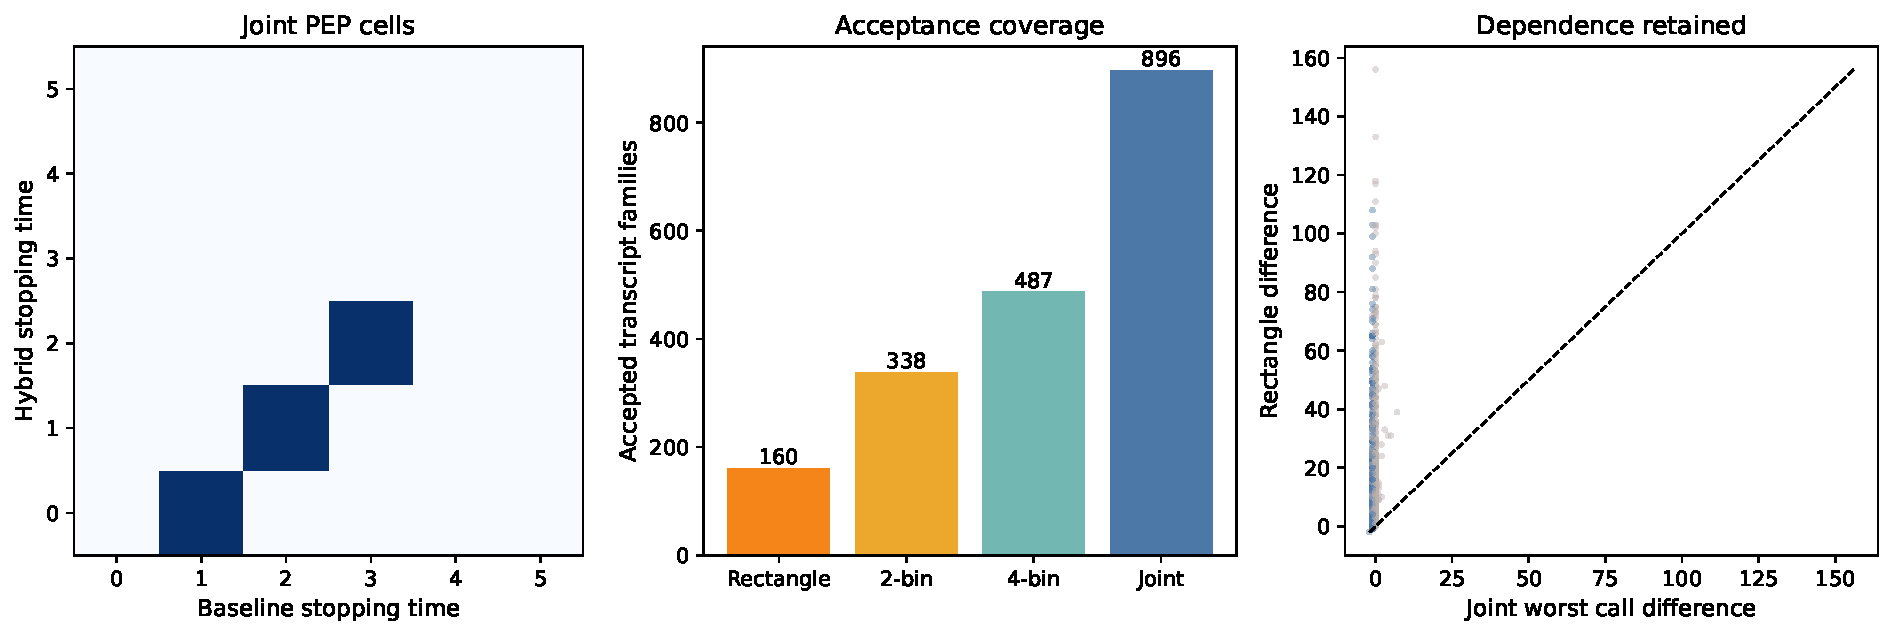
\includegraphics[width=\textwidth]{../figures/transcript_pep_study.pdf}
\caption{Left: positive-margin PEP cells in the analytic shift audit; boundary
cells within the numerical ambiguity threshold are not colored as attainable.
Center: acceptance coverage for one-, two-, and four-bin rectangles and the
full joint finite proxy.  Right: the
rectangular difference is never smaller than the joint difference and can be
substantially larger.}
\label{fig:audit}
\end{figure}

\subsection{Deterministic safety versus mean cost}

The preceding studies measure certificate structure, not whether deterministic
dominance is the best policy for an average-case objective.  To expose that
tradeoff rather than hide it, we bind a separate frozen accounting audit of
\AccountingCases{} dimension-64 diagonal quadratics.  Approximate-Newton
models have certified relative spectral errors, and proposal costs are sampled
from $\{0.25,0.5,1,2,4\}$ exact-call units.  The marginal pre-query gate uses
certified lower and upper call bounds; the always-query policy takes every
proposal without a dominance certificate.

\begin{table}[H]
\centering
\caption{Safety--mean tradeoff in the frozen accounting audit.  A total-cost
ratio above one is worse than the unchanged exact baseline.}
\label{tab:policy-accounting}
\begin{tabular}{lrrr}
\toprule
Policy & Mean ratio & Median ratio & Worse than baseline\\
\midrule
Exact only & 1.000 & 1.000 & 0.0\%\\
Certified marginal gate & \AccountingGateMeanRatio{} &
  \AccountingGateMedianRatio{} & 0.0\%\\
Always query & \AccountingAlwaysMeanRatio{} &
  \AccountingAlwaysMedianRatio{} & \AccountingAlwaysWorseRate{}\\
\bottomrule
\end{tabular}
\end{table}

The safe marginal gate accepts \AccountingGateAccepted{} cases
(\AccountingGateAcceptRate{}); accepted cases have mean ratio
\AccountingAcceptedMeanRatio{}, but rejected cases revert to ratio one, giving
the overall mean \AccountingGateMeanRatio{}.  Always querying has a much lower
mean ratio, \AccountingAlwaysMeanRatio{}, on this constructed distribution,
but is worse than exact-only in \AccountingAlwaysWorseRate{} of cases.  Thus
deterministic dominance is a tail-safety specification, not an estimator of the
mean-optimal policy.  If expected cost is the objective and distributional
risk is acceptable, a statistical or learning-augmented policy can rationally
prefer always querying.  \Cref{tab:joint-policy} benchmarks the joint gate on
the finite-family distribution.  The present ancillary audit uses a different,
more favorable approximate-Newton distribution and implements only the
rectangular gate; it quantifies a safety--mean tradeoff, not the joint gate's
relative conservatism.

\subsection{Real-SPX constant pipeline and application bridge}
\label{sec:real-spx}

The preceding experiments construct their constants.  To test whether the
constant interface can instead be made explicit and fully charged on observed
data, we use a frozen SPX option-chain snapshot with \RealSpxRawQuotes{} rows.
The snapshot was collected through \texttt{yfinance}; it is neither an official
consolidated feed nor evidence about another trading date.  A deterministic
filter retains \RealSpxFilteredQuotes{} native-OTM, liquid, positive noncrossed
quotes across \RealSpxExpiries{} expiries, with relative spread at most $8\%$,
$0.75\leq K/S\leq1.25$, $0.05\leq\mathrm{IV}\leq0.80$, and
$0.03\leq T\leq3$.

Let $X\in\mathbb Q^{n\times10}$ be a centered, scaled, and whitened
total-degree-three polynomial basis in moneyness and maturity, rounded at
$10^{-6}$, and let $v\in\mathbb Q^n$ be the similarly rounded implied
volatilities.  We solve the theorem-compatible quadratic
\[
 f(\theta)=\frac{1}{2n}\norm{X\theta-v}^2
          +\frac{1}{40}\norm{\theta}^2.
\]
The exact Hessian is $Q=X^\top X/n+(1/20)I$.  Rational Gershgorin arithmetic
gives $\mu=\RealSpxMu{}$ and $L=\RealSpxL{}$.  Starting from zero with
$\alpha=0.85/L$, the baseline stops after \RealSpxBaselineCalls{} exact
gradients.  The cheap candidate applies a Hessian built from every tenth quote
to the exact gradient already cached at the branch point.  Exact
\texttt{Fraction} replay verifies both strict threshold crossings and stops
after \RealSpxHybridCalls{} gradients, saving \RealSpxSavedCalls{}.

The cost conclusion changes when construction is charged.  One full-panel
gradient, cost $2nd$, is the unit.  The online sketch build, solve, and exact
quadratic replay cost \RealSpxOnlineCost{} units.  The declared one-time ledger
charges $50nd$ for filtering/features, $6nd^2$ for dense panel transforms, and
$30d^3$ for factorization and eigendecomposition, or
\RealSpxOfflineCost{} units.  Results are shown in
\cref{tab:real-constant-pipeline}.

\begin{table}[H]
\centering
\small
\caption{Real-SPX theorem-compatible surface: exact-call and complete declared
arithmetic-cost accounting.  The amortized row allocates the one-time pipeline
over the stated number of surfaces using the same preprocessing.}
\label{tab:real-constant-pipeline}
\begin{tabular}{lrr}
\toprule
Ledger & Exact-only units & Candidate-path units\\
\midrule
Exact calls only & \RealSpxBaselineCalls{}.000 & \RealSpxHybridCalls{}.000\\
Cold start, all declared arithmetic & \RealSpxBaselineCalls{}.000 &
  \RealSpxColdTotal{}\\
At \RealSpxBreakEven{} reuses & \RealSpxBaselineCalls{}.000 &
  \RealSpxWarmTotal{}\\
\bottomrule
\end{tabular}
\end{table}

Cold start therefore fails by a wide margin; the arithmetic ledger breaks even
only after \RealSpxBreakEven{} reuses.  A separate local CPU ledger is even
harsher.  Although online proposal plus replay measured
\RealSpxMeasuredCost{} exact-gradient times, CSV processing and exact rational
construction move measured break-even to \RealSpxMeasuredBreakEven{} reuses
because a ten-dimensional full-panel gradient is extremely cheap in optimized
NumPy.  These are environment-specific timings, not a theorem.  Their purpose
is to prevent the real-data example from hiding the very constant-acquisition
cost it is meant to expose.

\subsubsection{A positive ill-conditioned acceptance}
The whitened surface is a deliberately harsh control because the exact
baseline already converges in seven calls.  We therefore repeat the study on
the same \RealSpxFilteredQuotes{} quotes after centering and RMS scaling but
\emph{without} whitening, and reduce the ridge to $10^{-4}$.  The resulting
rational Hessian is no longer close to a multiple of the identity.  Exact
leading-principal-minor checks prove
\[
  \frac{1}{400}I \prec Q \prec \frac{21}{5}I.
\]
Integer minimum- and maximum-mode Rayleigh witnesses independently prove the
stronger lower condition bound, giving the certified interval
\[
  \PositiveSpxConditionLower{} < \kappa(Q) <
  \PositiveSpxConditionUpper{}.
\]
The baseline uses $\alpha=17/84$ and requires
\PositiveSpxBaselineCalls{} full-panel gradients.  The same every-tenth-quote
sketch, applied to the cached exact gradient, requires
\PositiveSpxHybridCalls{}, a saving of \PositiveSpxSavedCalls{} calls.

The stopping counts are not floating classifications.  A standard-library
verifier, whose code is not imported by the generator, checks the exact
rational sketch identity $M y=b$, both strict curvature matrices by their
leading minors, both Rayleigh witnesses, and the complete arithmetic-cost
ledger.  It then evaluates $g_k=(I-\alpha Q)^k g_0$ by 110-digit,
directed-rounding Decimal
interval matrix powers.  The two intervals straddle neither side of the
stopping threshold at $N-1$ and $N$.  Since
$0<\alpha\lambda(Q)<1$, gradient norms decrease monotonically, so these two
crossings certify the exact stopping times.  When the companion market
snapshot is supplied, the verifier additionally rebuilds the data-to-matrix
map independently and matches the rational matrices exactly.  Rehashed
perturbations of the candidate, a curvature minor, a stopping count, and a
cost-ledger entry are all rejected.  Wall-clock timings remain descriptive
measurements rather than verified certificate fields.

\begin{table}[H]
\centering
\small
\caption{Positive real-SPX acceptance.  Nonexact cost includes the full
filter/feature and full/sketch Gram pipelines, curvature work, proposal solve,
and a conservative sequential-replay charge under the same
$50nd+6nd^2+30d^3$ ledger as the whitened control, all in full-panel gradient
units.}
\label{tab:positive-real-spx}
\begin{tabular}{lrrrr}
\toprule
Path & Exact calls & Charged nonexact & Total units & Ratio\\
\midrule
Exact only & \PositiveSpxBaselineCalls{} & 0 &
  \PositiveSpxBaselineCalls{} & 1.000\\
Certified candidate & \PositiveSpxHybridCalls{} &
  \PositiveSpxNonexactCost{} & \PositiveSpxCandidateTotal{} &
  \PositiveSpxCostRatio{}\\
\bottomrule
\end{tabular}
\end{table}

Thus the gate accepts with \PositiveSpxCostSlack{} units of cost slack even at
cold start.  In three local repeats the one-time pipeline, including
certificate generation and independent verification, took
\PositiveSpxPipelineSeconds{} seconds.  It breaks even after
\PositiveSpxBreakEven{} uses; at that point the measured total ratio is
\PositiveSpxMeasuredRatio{}, while the warm-path speedup is
$\PositiveSpxWarmSpeedup{}\times$.  Timing is machine specific, but the exact
identities and arithmetic ledger are not.  This is a positive real-market,
far-from-unit-condition data point.  Its transcript reveals the full rational
quadratic $(Q,b)$, so it is not a claim that a short first-order transcript
would certify the same acceptance, nor is it a nonlinear calibration result.

To quantify what remains after removing full $(Q,b)$ revelation, retain only
the cached gradient, candidate vector, and certified
$\mu=1/400$, $L=21/5$.  The smooth lower residual factor
$1-\alpha L=0.15$ certifies only
$N_f(x)\geq\PositiveSpxShortBaselineLower{}$, whereas distance contraction
gives the candidate upper bound
$N_f(y)\leq\PositiveSpxShortHybridUpper{}$.  The resulting marginal screen is
decisively uncertified, and a joint enumeration at that horizon was not
attempted.  Thus the \PositiveSpxCostRatio{} full-model ratio disappears as a
PEP acceptance claim when $(Q,b)$ is hidden; what remains is evidence that the
constant interface and common cost ledger can be audited on market data.

We also freeze a $3\times3\times3$ sensitivity grid over ridge
$\{10^{-5},10^{-4},10^{-3}\}$, sketch stride $\{5,10,20\}$, and relative
squared tolerance $\{10^{-8},10^{-10},10^{-12}\}$.  All
\SpxSensitivityAccepted{} of \SpxSensitivityConfigurations{} deliberately
reported configurations pass the common ledger, with total ratios from
\SpxSensitivityMinRatio{} to \SpxSensitivityMaxRatio{} and saved-call counts
from \SpxSensitivityMinSaved{} to \SpxSensitivityMaxSaved{}.  The base ratio
under this unified ledger is \SpxSensitivityBaseRatio{}.  Exact leading-minor
checks additionally show that conservative declarations $\mu=1/800$ and
$L=231/50$ remain valid, while optimistic declarations $\mu=1/200$ and
$L=189/50$ fail.  Consequently curvature mis-specification is not treated as
benign: an optimistic bound moves the instance outside the certified
transcript rather than producing an accepted sensitivity point.

An out-of-class $101\times101$ projected nonconvex SLV calibration remains in
the artifact as a descriptive downstream stress record, but its former table
is removed: it used more exact adjoints and supplies no evidence for the
theorems or the two-oracle gate.

\section{Implementation limits and extensions}

The certificate is exact only relative to what is declared.  If a cheap error
contract is false, the function lies outside $\mathfrak F(\cT)$ and the claim
does not apply.  If the physical dimension is smaller than the Gram rank, the
dimension-free SDP is conservative unless the rank constraint is enforced.
If no finite distance or residual bound is available, the stopping grid may be
unbounded.  If certificate computation costs more than the calls it certifies,
the candidate cannot be accepted after that cost is included; an online return
to the unchanged baseline still requires the funding condition
\eqref{eq:fallback}.  The construction in
\cref{prop:transcript-pipeline} makes $R,D,\delta$ auditable when a gradient and
$\mu$ are already certified; it does not show that global curvature or interval
constants are cheap to obtain in every application.  The real-SPX surface in
\cref{sec:real-spx} supplies such pipelines and charges them.  The whitened
control fails at cold start, whereas the ill-conditioned surface in
\cref{tab:positive-real-spx} pays the full ledger immediately because the
exact baseline has thousands of calls left.  The positive SPX transcript
reveals the full rational $(Q,b)$.  The nonquadratic example above shows that a
genuinely short, non-shift first-order transcript can suffice when the
certified curvature interval is tight; its realized trajectory spans $\R^2$,
its natural certified horizon is two, and its exact SDP audit is deliberately
padded to horizon three.  Obtaining comparably tight low-cost constants from short
transcripts in large nonlinear applications remains the principal practical
bottleneck.

The intended operating regime is consequently narrow: high-fidelity calls
must be expensive black-box operations, proposal and proof work must be
prepaid or reusable, and the curvature, distance, oracle-contract, and cost
constants must themselves be certifiable.  The architecture is not
economically justified for a one-off branch with millisecond gradients, nor
when obtaining global constants reveals essentially the whole model.  For the
full-model SPX quadratic, realistic reuse could arise from repeated surfaces
sharing a fixed feature map and maturity panel, but the present snapshot does
not establish a production reuse distribution; its result remains a stress
test of the accounting interface.

The exact-shift audit in \cref{tab:scaling} reduces the residual SDP count from
quadratic to linear in $H$.  The ragged audit in
\cref{tab:generic-scaling} removes that identity and solves every
cost-violating cell at $H=20$, but it is a floating-point diagnostic whose
proof-carrying outcome is \emph{uncertified}.  Acceptance would require
independently validated dual exclusions for all \GenericPepBadCells{} bad
cells.  The nonlinear example instead recovers and independently verifies
ordinary rational Gram-SDP duals for all ten cells in a padded $H=3$ audit of
an $H_0=2$ transcript, with 100 exact
positive-minor checks.  The analytic contraction argument is retained only as
an independent cross-check.  This closes the missing small-scale end-to-end
path, not generic dual recovery at $H=20$.  Longer
horizons, full attainable-set reconstruction, and exact generic dual recovery
at scale remain computational limitations.

Three extensions appear especially worthwhile but are not claimed here.
First, operator interpolation could couple primal--dual or proximal
continuations \citep{Bousselmi2024}.  Second, a local active-face transcript
could condition the PEP after identification, provided the face-stability
certificate itself is exact.  Third, chordal sparsity, cell dominance, and
validated dual reconstruction could make proof-carrying certificates practical
at longer horizons.  Adaptive step sizes and line searches would additionally
make each stopping cell depend on the realized step and acceptance history, so
they require new interpolation variables and coupling constraints rather than
a mechanical reuse of the fixed-step grid.  Each extension changes the
interpolation or computational backend and is outside the verified fixed-step
implementation studied here.

\section{Conclusion}

C2OGate turns a one-shot proposal-versus-baseline branch decision into a
proof-carrying computational
workflow.  The method retains the joint dependence between baseline and
candidate stopping times, generates only the cost-violating cells, screens
them with auditable identities, and separates numerical search from the proof
required for acceptance.  Its three-valued output is deliberate: a witnessed
bad cell rejects, verified exclusion of every bad cell can accept, and every
remaining numerical or modeling uncertainty is reported as uncertified.

For fixed-step gradient descent on $\cF_{\mu,L}$, the finite-horizon and Gram
constructions make this workflow exact in the dimension-free setting, with a
rank qualification for fixed dimension.  The experiments demonstrate both
sides of the interface: structure reduces a horizon-20 run from 441 nominal
cells to 20 SDP solves; a generic horizon-20 audit remains uncertified rather
than promoting floating statuses to proofs; and a non-shift, nonquadratic
two-dimensional acceptance with natural horizon $H_0=2$ is carried by ten
recovered and independently verified generic PEP duals on a padded $H=3$
grid.  The finite-family study is a constructed proxy, and the real-SPX
result is a full-model constant-pipeline stress test whose short-transcript
screen does not accept.  The evidence therefore does not establish universal
acceleration, cheap constant acquisition, or scalable exact dual recovery.  It
establishes a conservative implementation pattern for making and auditing
cost-dominance claims when the function class, transcript, oracle contract,
dimension, funding source, and cost units can themselves be certified.

\bibliographystyle{spmpsci}
\bibliography{references}

\section*{Statements and Declarations}

\paragraph{Funding}
The author declares that no funds, grants, or other support were received
during the preparation of this manuscript.

\paragraph{Competing interests}
The author has no relevant financial or non-financial interests to disclose.

\paragraph{Author contributions}
Jintao Li performed the conceptualization, methodology, software development,
formal analysis, validation, data curation, visualization, and writing, and
approved the submitted manuscript.

\paragraph{Data availability}
The submission archive contains the frozen hash-bound JSON records used for
every reported claim.  These derived records are the self-contained
reproduction units.  Raw SPX rows are not redistributed because they originate
from an unofficial third-party market snapshot; the expected source hash and
the independent data-to-matrix reconstruction procedure are documented.
Accordingly, a clean checkout supports certificate \emph{replay} and every
paper/table integrity check, but not raw-data-to-matrix \emph{regeneration} of
the SPX studies unless the matching external snapshot is supplied.

\paragraph{Code availability}
The C2OGate source, experiment drivers, exact rational certificates,
standard-library verifiers, unit and integrity tests, and manuscript build
scripts are publicly available under the MIT License at
\url{https://github.com/LiGentle/C2OGate}.  A clean checkout can replay every
frozen certificate and rebuild the manuscript without the raw market
snapshot.

\paragraph{Use of generative artificial intelligence}
OpenAI Codex was used to assist with software development, computational
checking, and manuscript drafting.  The author reviewed the resulting code,
proofs, experiments, and text and takes full responsibility for the submitted
work.

\appendix

\section{Explicit Gram coefficients}
\label{app:gram}

For completeness, let $v_1,\ldots,v_p$ be the vector atoms and associate a
coefficient vector $a(z)\in\R^p$ with every sampled point or gradient, so that
$z=\sum_{\ell=1}^p a_\ell(z)v_\ell$.  Then
\begin{equation}
 \ip{u}{v}=a(u)^\top G a(v),\qquad
 \norm{u-v}^2=(a(u)-a(v))^\top G(a(u)-a(v)).
 \label{eq:gram-coeff}
\end{equation}
With $a(x)=0$, $a(y)$ an atom, and $a(g_k^x),a(g_k^y)$ gradient atoms,
the recurrence coefficients are
\begin{align*}
 a(x_k)&=-\alpha\sum_{t=0}^{k-1}a(g_t^x),\\
 a(y_k)&=a(y)-\alpha\sum_{t=0}^{k-1}a(g_t^y).
\end{align*}
Substitution of \eqref{eq:gram-coeff} into
\eqref{eq:interpolation} makes every term affine in $G$.  For example,
contract \eqref{eq:cheap-contract} is
\[
 (a(y)+\gamma a(g_0^x))^\top G
 (a(y)+\gamma a(g_0^x))\leq\delta^2.
\]
The distance bound is
$a(x_*)^\top G a(x_*)\leq R^2$, and each stopping constraint is a diagonal
quadratic form $a(g)^\top G a(g)\lesseqgtr\eps^2$ with the appropriate margin.
This is the complete algebra used by the implementation.

\section{Reproducibility record}
\label{app:repro}

The frozen payload hash is
\begin{center}
\small\nolinkurl{\TranscriptPayloadHash}.
\end{center}
The frozen accounting-audit payload hash is
\begin{center}
\small\nolinkurl{\AccountingPayloadHash}.
\end{center}
The frozen PEP-scaling payload hash is
\begin{center}
\small\nolinkurl{\PepScalingPayloadHash}.
\end{center}
The frozen generic non-shift PEP payload hash is
\begin{center}
\small\nolinkurl{\GenericPepPayloadHash}.
\end{center}
The independently verified generic nonquadratic PEP-dual payload hash is
\begin{center}
\small\nolinkurl{\GenericDualPayloadHash}.
\end{center}
The independently verified nonquadratic acceptance payload hash is
\begin{center}
\small\nolinkurl{\NonlinearPepPayloadHash}.
\end{center}
The frozen real-SPX bridge payload hash is
\begin{center}
\small\nolinkurl{\RealSpxPayloadHash}.
\end{center}
The independently verified positive real-SPX payload hash is
\begin{center}
\small\nolinkurl{\PositiveSpxPayloadHash}.
\end{center}
Its out-of-class production source payload hash is
\begin{center}
\small\nolinkurl{\ProductionPayloadHash}.
\end{center}
The independently verified rational-certificate payload hash is
\begin{center}
\small\nolinkurl{\RationalCertificatePayloadHash}.
\end{center}
The measured certificate-cost payload hash is
\begin{center}
\small\nolinkurl{\CertificateCostPayloadHash}.
\end{center}
The frozen SPX sensitivity payload hash is
\begin{center}
\small\nolinkurl{\SpxSensitivityPayloadHash}.
\end{center}
The study is regenerated by
\begin{verbatim}
make transcript-study
\end{verbatim}
The structure-exploiting scaling audit is regenerated by
\begin{verbatim}
make pep-scaling-study
\end{verbatim}
The generic non-shift enumeration and the real-SPX study are regenerated by
\begin{verbatim}
make generic-pep-scaling-study
make generic-pep-dual
make nonlinear-pep-acceptance
make real-spx-study
make real-spx-positive-study
make certificate-cost-study
make spx-sensitivity-study
\end{verbatim}
The frozen, hash-bound JSON payloads are the self-contained reproduction units
for certificate replay, the test suite, and manuscript compilation.  Raw
market regeneration is a separate operation: the unofficial SPX snapshot and
the upstream SLV audit are not redistributed with this repository.  With the
repository located at
\nolinkurl{<companion-root>/two_oracle_cost_gate}, both real-SPX regeneration
targets require the CSV and metadata under
\nolinkurl{<companion-root>/data/market_data/}.  The whitened bridge
additionally requires the hash-bound production payload under
\nolinkurl{<companion-root>/HWC_study/production_real/}.  These external files
and their expected hashes are recorded in the payload and README.  Thus a
clean checkout can replay every frozen certificate and build this paper,
whereas rebuilding the market-derived matrices requires the named companion
snapshot.  Supplying it to the positive verifier via
\texttt{--source-root} triggers an independent data-to-matrix reconstruction.
The safety--mean accounting audit is regenerated by
\begin{verbatim}
make study
\end{verbatim}
The high-precision proposals are regenerated and then exactly verified by
\begin{verbatim}
make rational-certificates
\end{verbatim}
and the manuscript by
\begin{verbatim}
make mpc-paper
\end{verbatim}
The integrity test recomputes the canonical JSON hash, checks the runner and
all recorded source hashes, verifies the frozen counts in \cref{tab:audit}, and
checks that no rectangular acceptance lies outside the joint acceptance set.
It also recomputes every realized-member cost in \cref{tab:joint-policy}.
The complete PEP cell margins, including all four near-zero cells, remain in
the payload rather than being rounded away in the paper.  The accounting
integrity test checks every value reported in \cref{tab:policy-accounting} and
zero accepted dominance violations.  Scaling integrity tests check every
enumeration count in \cref{tab:scaling,tab:generic-scaling}, the largest Gram
orders, all bad-cell records, and runner hashes.  The real-data test replays
both stopping times in exact rational arithmetic, recomputes the Gershgorin
bounds and strict crossings, verifies both cost ledgers, and follows the hash
chain into the production payload.  A separate integrity test binds the
rational dual payload to its generator and verifier, checks the counts in
\cref{tab:rational-certificates}, and exercises adversarial rehashed slack and
witness tampering.  The generic-dual test reconstructs all ten rational Gram
SDPs, verifies 100 positive leading minors, and exercises rehashed changes to
the transcript, a cell identity, a dual multiplier, a Gram coefficient, and a
principal minor.  The nonlinear-acceptance test
independently recomputes the realized transcendental gradients, every rational
contraction bound, the ten bad cells, and the joint cost inequality; four
rehashed tampering tests alter the candidate, a bound, a cell record, and the
charged cost.  The positive
real-SPX verifier independently checks exact
candidate and curvature identities, rational condition witnesses,
directed-rounding stopping intervals, and the full arithmetic-cost ledger;
when the companion snapshot is present it also reconstructs the matrices from
the raw rows.  Its tests rehash and perturb the candidate, a leading minor, a
stopping count, and a cost entry.

\end{document}
